% ------------------------------------------------------------------------
% ------------------------------------------------------------------------
% Modelo UFSC para Trabalhos Academicos (tese de doutorado, dissertação de
% mestrado) utilizando a classe abntex2
%
% Autor: Alisson Lopes Furlani
% 	Modificações:
%	- 27/08/2019: Alisson L. Furlani, add 'glossaries' package
%   - 30/10/2019: Alisson L. Furlani, adjusted some spacing errors and changed math fonts
%   - 17/01/2020: Alisson L. Furlani, updated certification page
%   - 07/02/2020: Alisson L. Furlani, fixed table counter bug
%   - 11/03/2020: Alisson L. Furlani, changed greek letters in math and fixed citation style
%   - 14/09/2020: Alisson L. Furlani, little adjustments
%   - 30/08/2021: Alisson L. Furlani, add glossaries
% ------------------------------------------------------------------------
% ------------------------------------------------------------------------

\documentclass[
	% -- opções da classe memoir --
	12pt,				% tamanho da fonte
	%openright,			% capítulos começam em pág ímpar (insere página vazia caso preciso)
	oneside,			% para impressão no anverso. Oposto a twoside
	a4paper,			% tamanho do papel. 
	% -- opções da classe abntex2 --
	chapter=TITLE,		% títulos de capítulos convertidos em letras maiúsculas
	section=TITLE,		% títulos de seções convertidos em letras maiúsculas
	%subsection=TITLE,	% títulos de subseções convertidos em letras maiúsculas
	%subsubsection=TITLE,% títulos de subsubseções convertidos em letras maiúsculas
	% -- opções do pacote babel --
	english,			% idioma adicional para hifenização
	%french,				% idioma adicional para hifenização
	%spanish,			% idioma adicional para hifenização
	brazil				% o último idioma é o principal do documento
	]{abntex2}

\usepackage{setup/ufscthesisA4-alf}

%%\usepackage{algorithmic}
%\usepackage{algorithm}
%\usepackage[noend]{algpseudocode}
%\usepackage{textcomp}
%\usepackage{amssymb}
%\usepackage{amsmath}


\SetKwProg{procedure}{procedure}{}{}
\SetKwProg{when}{when}{}{}
\SetKwProg{foreach}{for each}{}{}
\SetKwProg{while}{while}{}{}

\addbibresource{aftertext/references.bib}

% ajusta espaçamento das listas itemize e enumerate
\setitemize{topsep=0pt,itemsep=0pt,leftmargin=\parindent+\labelwidth-\labelsep}
\setenumerate{topsep=0pt,itemsep=0pt,leftmargin=\parindent+\labelwidth-\labelsep}

% define a macro \Autoref to allow multiple references to be passed to \autoref
\makeatletter
\newcommand\Autoref[1]{\@first@ref#1,@}
\def\@throw@dot#1.#2@{#1}% discard everything after the dot
\def\@set@refname#1{%    % set \@refname to autoefname+s using \getrefbykeydefault
	\edef\@tmp{\getrefbykeydefault{#1}{anchor}{}}%
	\xdef\@tmp{\expandafter\@throw@dot\@tmp.@}%
	\ltx@IfUndefined{\@tmp autorefnameplural}%
	{\def\@refname{\@nameuse{\@tmp autorefname}s}}%
	{\def\@refname{\@nameuse{\@tmp autorefnameplural}}}%
}
\def\@first@ref#1,#2{%
	\ifx#2@\autoref{#1}\let\@nextref\@gobble% only one ref, revert to normal \autoref
	\else%
	\@set@refname{#1}%  set \@refname to autoref name
	\@refname~\ref{#1}% add autoefname and first reference
	\let\@nextref\@next@ref% push processing to \@next@ref
	\fi%
	\@nextref#2%
}
\def\@next@ref#1,#2{%
	\ifx#2@ e~\ref{#1}\let\@nextref\@gobble% at end: print e+\ref and stop
	\else, \ref{#1}% print  ,+\ref and continue
	\fi%
	\@nextref#2%
}
\makeatother

% Cria comando para referenciar Anexo automaticamente \refanexo
\newcommand{\refanexo}[1]{\hyperref[#1]{Anexo~\ref{#1}}}

% Define comandos para tabelas que permite ajustar o tamanho da coluna e manter alinhamento C, R ou L
%\newcommand{\PreserveBackslash}[1]{\let\temp=\\#1\let\\=\temp}
\newcolumntype{C}[1]{>{\centering\let\arraybackslash}m{#1}}
\newcolumntype{R}[1]{>{\RaggedLeft\let\arraybackslash}m{#1}}
\newcolumntype{L}[1]{>{\RaggedRight\let\arraybackslash}m{#1}}

\newcommand\tstrut{\rule{0pt}{2.4ex}}
\newcommand\bstrut{\rule[-1.0ex]{0pt}{0pt}}
% ---
% Filtering and Mapping Bibliographies
% ---
\DeclareSourcemap{
	\maps[datatype=bibtex]{
		% remove fields that are always useless
		\map{
			\step[fieldset=abstract, null]
			\step[fieldset=pagetotal, null]
			\step[fieldset=doi, null]
		}
		% remove URLs for types that are primarily printed
		\map{
			\pernottype{software}
			\pernottype{online}
			\pernottype{report}
			\pernottype{techreport}
			\pernottype{standard}
			\pernottype{manual}
			\pernottype{misc}
			\step[fieldset=url, null]
			\step[fieldset=urldate, null]
		}
		\map{
			\pertype{inproceedings}
			% remove mostly redundant conference information
			%\step[fieldset=venue, null]
			%\step[fieldset=eventdate, null]
			%\step[fieldset=eventtitle, null]
			% do not show ISBN for proceedings
			\step[fieldset=isbn, null]
			% Citavi bug
			%\step[fieldset=volume, null]
		}
	}
}
% ---

\definecolor{cadmiumgreen}{rgb}{0.0, 0.42, 0.24}
\definecolor{burntorange}{rgb}{0.8, 0.33, 0.0}
\definecolor{green}{rgb}{0,0.5,0}
%\definecolor{purple}{rgb}{0.59,0.44,0.84}
\definecolor{purple}{rgb}{1,0.2,1}
\definecolor{dodgerblue}{rgb}{0.1,0.6,1}
\definecolor{royalblue}{rgb}{0.2,0.4,0.8}


\newcommand{\ct}[1]{{\color{red}#1}}
% final version - uncomment line below and comment line above
%\newcommand{\ct}[1]{}

\newcommand{\odo}[1]{{\color{burntorange}#1}}
% final version - uncomment line below and comment line above
%\newcommand{\odo}[1]{{\color{black}#1}}

\newcommand{\lucas}[1]{{\color{cadmiumgreen}#1}}
% final version - uncomment line below and comment line above
%\newcommand{\lucas}[1]{{\color{black}#1}}




% ---
% Informações de dados para CAPA e FOLHA DE ROSTO
% ---
% FIXME Substituir 'Nome completo do autor' pelo seu nome.
\autor{Lucas Pagotto Tonussi}
% FIXME Substituir 'Título do trabalho' pelo título da trabalho.
\titulo{Estendendo um Ordenador de Mensagens em Arquitetura de Microsserviços para Comunicação sobre o Protocolo HTTP}
% FIXME Substituir 'Subtítulo (se houver)' pelo subtítulo da trabalho.  
% Caso não tenha substítulo, comente a linha a seguir.
\subtitulo{}
% FIXME Substituir 'XXXXXX' pelo nome do seu
% orientador.
\orientador{Prof. Odorico Machado Mendizabal, Dr.}
% FIXME Se for orientado por uma mulher, comente a linha acima e descomente a linha a seguir.
% \orientador[Orientadora]{Nome da orientadora, Dra.}
% FIXME Substituir 'XXXXXX' pelo nome do seu
% coorientador. Caso não tenha coorientador, comente a linha a seguir.
% \coorientador{Prof. XXXXXX, Dr.}
% FIXME Se for coorientado por uma mulher, comente a linha acima e descomente a linha a seguir.
% \coorientador[Coorientadora]{XXXXXX, Dra.}
% FIXME Substituir '[ano]' pelo ano (ano) em que seu trabalho foi defendido.
\ano{2022}
% FIXME Substituir '[dia] de [mês] de [ano]' pela data em que ocorreu sua defesa.
%\data{[dia] de [mês] de [ano]}
% FIXME Substituir 'Local' pela cidade em que ocorreu sua defesa.
\local{Florianópolis (SC)}
\instituicaosigla{UFSC}
\instituicao{Universidade Federal de Santa Catarina}
% FIXME Substituir 'Dissertação/Tese' pelo tipo de trabalho (Tese, Dissertação). 
\tipotrabalho{Monografia}
% FIXME Substituir '[mestre/doutor] em XXXXXX' pela grau adequado.
\formacao{Bacharel em Sistemas de Informação}
% FIXME Substituir '[mestrado/doutorado]' pelo nivel adequado.
% \nivel{[mestrado/doutorado]}
% FIXME Substituir 'Programa de Pós-Graduação em XXXXXX' pela curso adequado.
\programa{Bacharelado em Sistemas de Informação}
% FIXME Substituir 'Campus XXXXXX ou Centro de XXXXXX' pelo campus ou centro adequado.
\centro{Campus Florianópolis}
\preambulo
{%
\imprimirtipotrabalho~submetida~ao~\imprimirprograma~da~\imprimirinstituicao~para~a~obtenção~do~título~de~\imprimirformacao.
}
% ---

% ---
% Configurações de aparência do PDF final
% ---
% alterando o aspecto da cor azul
\definecolor{blue}{RGB}{41,5,195}
% informações do PDF
\makeatletter
\hypersetup{
%pagebackref=true,
pdftitle={\@title}, 
pdfauthor={\@author},
pdfsubject={\imprimirpreambulo},
pdfcreator={LaTeX with abnTeX2},
pdfkeywords={ufsc, latex, abntex2}, 
colorlinks=true,       		% false: boxed links; true: colored links
linkcolor=black,%blue,          	% color of internal links
citecolor=black,%blue,        		% color of links to bibliography
filecolor=black,%magenta,      		% color of file links
urlcolor=black,%blue,
bookmarksdepth=4
}
\makeatother
% ---

% ---
% compila a lista de abreviaturas e siglas e a lista de símbolos
% ---

% Declaração das siglas
\siglalista{ABNT}{Associação Brasileira de Normas Técnicas}
\siglalista{RME}{Replicação por Máquina de Estados}
\siglalista{RMEP}{Replicação por Máquina de Estados Paralela}
\siglalista{SBC}{Sociedade Brasileira de Computação}
\siglalista{LaPeSD}{Laboratório de Pesquisa em Sistemas Distribuídos}
\siglalista{TCC}{Trabalho de Conclusão de Curso}
\siglalista{ACM}{\textit{Association for Computing Machinery}}
\siglalista{UDP}{\textit{User Datagram Protocol}}
\siglalista{GRPC}{\textit{Google Remote Procedure Call}}
\siglalista{CRDT}{\textit{Conflict-free Replicated Data Types}}
\siglalista{SOC}{Software de Orquestração de Contêineres}
\siglalista{K8S}{Kubernetes}
\siglalista{DevOps}{Desenvolvimento e Operações}
\siglalista{API}{\textit{Application Programming Interface}}
\siglalista{UCP}{Unidade Central de Processamento}
\siglalista{FIFO}{\textit{First In First Out}}
\siglalista{UML}{\textit{Unified Modelling Language}}
\siglalista{AB-cast}{\textit{Atomic Broadcast}}
\siglalista{CPU}{\textit{Central Processing Unit}}
\siglalista{HTTP}{\textit{Hypertext Transfer Protocol}}
\siglalista{IEEE}{\textit{Institute of Electrical and Electronics Engineers}}
\siglalista{RWO}{\textit{Read Write Once}}
\siglalista{ROX}{\textit{Read Only Many}}
\siglalista{RWX}{\textit{Read Write Many}}
\siglalista{RWOP}{\textit{Read Write Once Pod}}
\siglalista{IP}{\textit{Internet Protocol}}
\siglalista{ASCII}{\textit{American Standard Code for Information Interchange}}
%\newacronym[user1=\emph{english}]{pt}{pt}{portugues}
%\newacronym[\glslongpluralkey={siglas}]{s}{s}{sigla}

% Declaração dos simbolos
% \simbololista{C}{\ensuremath{C}}{Circunferência de um círculo}
% \simbololista{pi}{\ensuremath{\pi}}{Número pi} 
% \simbololista{r}{\ensuremath{r}}{Raio de um círculo}
% \simbololista{A}{\ensuremath{A}}{Área de um círculo}

% Declaração de acrônimos
% \glossariolista{Palavra}{Descrição da palavra... escrevendo aqui para ocupar mais de uma linha e testar o template}
% \glossariolista{OutraPalavra}{Descrição da outra palavra}

% ###################################
% ###################################
% ################################### OS OUTROS GLOSSÁRIOS NÃO ESTÃO COMPILANDO
% ###################################
% ###################################

% \glossariolista{Pod}{Um \textit{pod} do Kubernetes é um conjunto de um ou mais contêineres, sendo a menor unidade de uma aplicação Kubernetes.}
% \glossariolista{Api}{API é uma sigla para Application Programming Interface, ou seja, é um conjunto de definições e protocolos para construção e integração de aplicações de software.}
% \glossariolista{Microsserviço}{Microsserviço é uma arquitetura de software na qual o software consiste de uma aplicação independente, isolada, escalável, re-programável ou, substituível sem que isso afete outras partes.}


% compila a lista de abreviaturas e siglas e a lista de símbolos
\makenoidxglossaries 

% ---

% ---
% compila o indice
% ---
\makeindex
% ---

% ----
% Início do documento
% ----
\begin{document}

% Seleciona o idioma do documento (conforme pacotes do babel)
%\selectlanguage{english}
\selectlanguage{brazil}

% Retira espaço extra obsoleto entre as frases.
\frenchspacing 

% Espaçamento 1.5 entre linhas
\OnehalfSpacing

% Corrige justificação
%\sloppy

% ----------------------------------------------------------
% ELEMENTOS PRÉ-TEXTUAIS
% ----------------------------------------------------------
% \pretextual %a macro \pretextual é acionado automaticamente no início de \begin{document}
% ---
% Capa, folha de rosto, ficha bibliografica, errata, folha de apróvação
% Dedicatória, agradecimentos, epígrafe, resumos, listas
% ---
\imprimircapa

\imprimirfolhaderosto*

% http://ficha.bu.ufsc.br/
\begin{fichacatalografica}
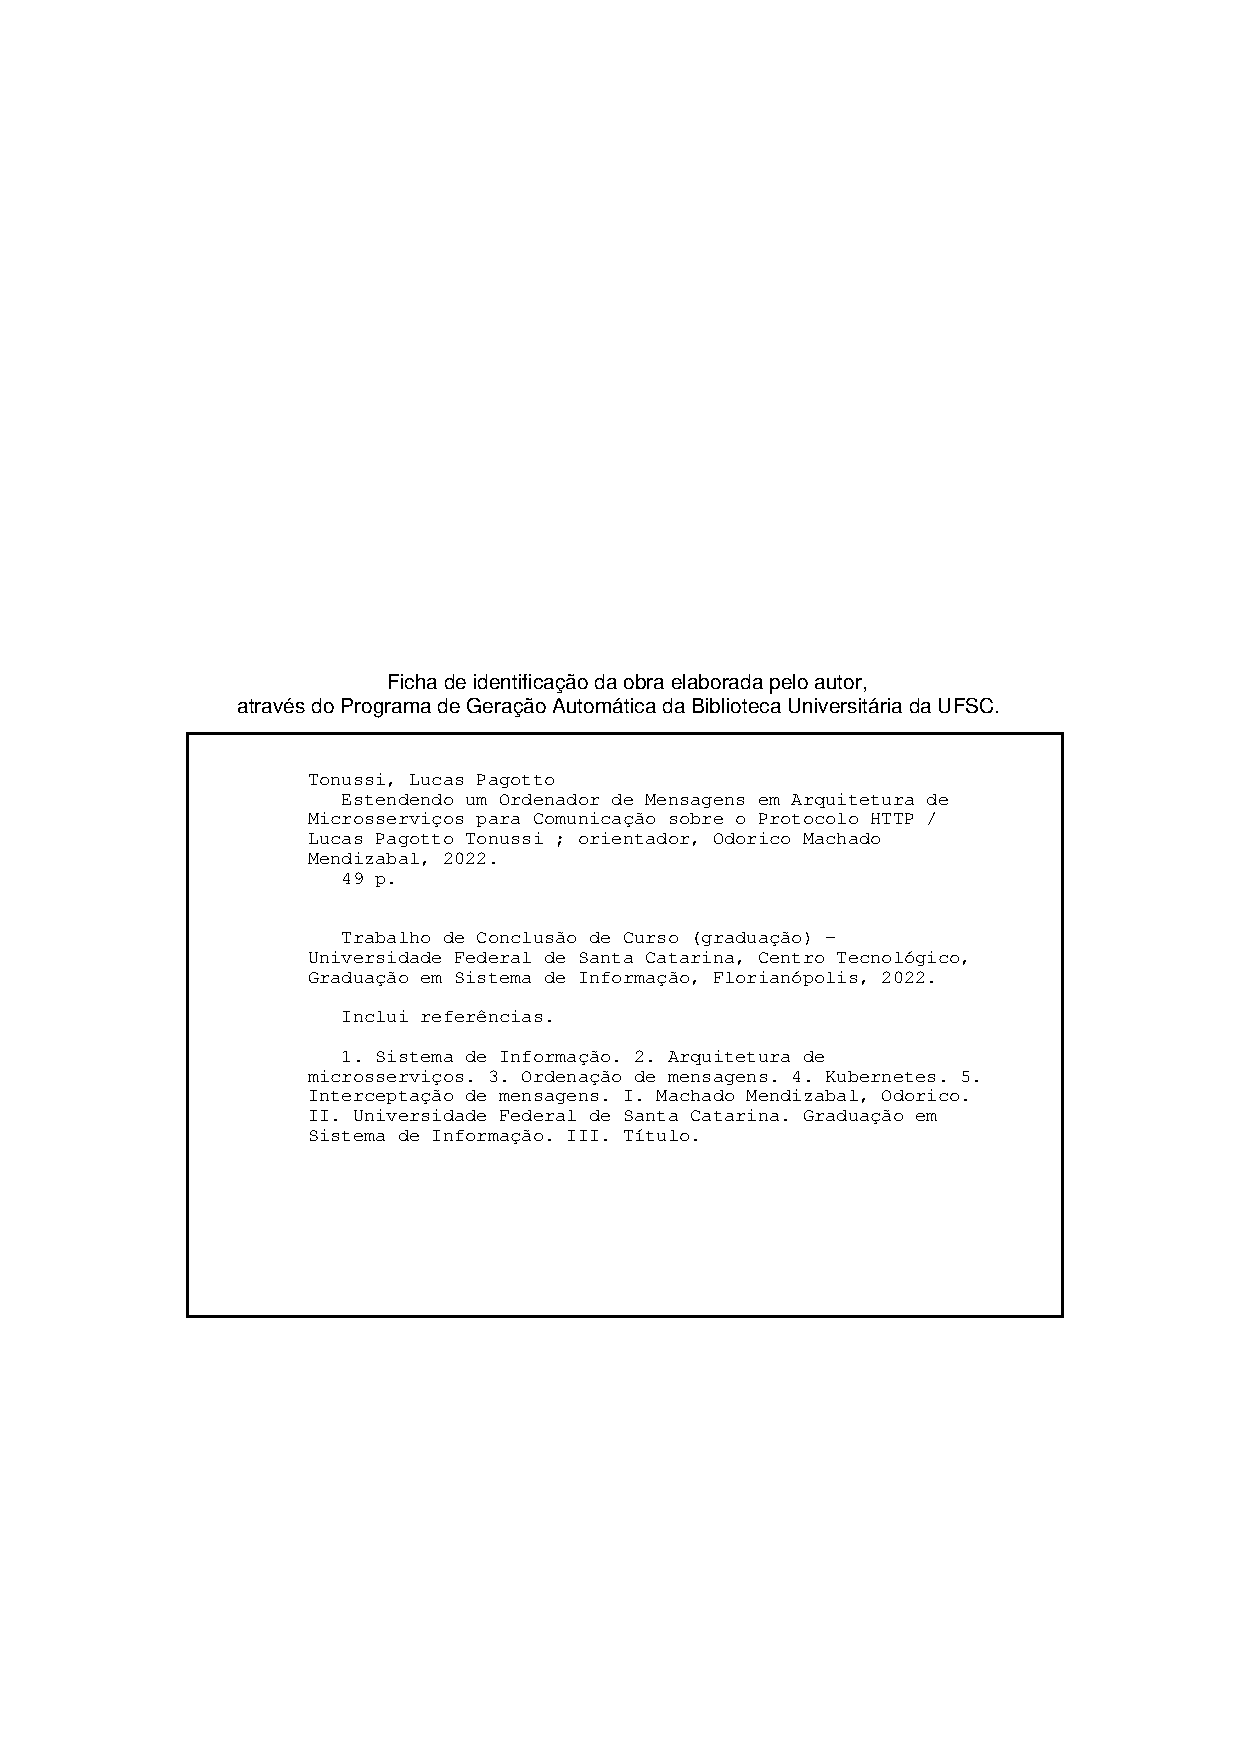
\includepdf{beforetext/Ficha_Catalografica_Preenchido.pdf}
\end{fichacatalografica}

\begin{folhadeaprovacao}
\OnehalfSpacing
\centering
\imprimirautor\\%
\vspace*{10pt}		
\textbf{\imprimirtitulo}%
\ifnotempty{\imprimirsubtitulo}{:~\imprimirsubtitulo}\\%
% \vspace*{31.5pt}%3\baselineskip
\vspace*{\baselineskip}
%\begin{minipage}{\textwidth}
O presente trabalho em nível de \imprimirnivel~foi avaliado e aprovado por banca examinadora composta pelos seguintes membros:\\
%\end{minipage}%
\vspace*{\baselineskip}
Prof.(a) Luciana de Oliveira Rech, Dr(a).\\
Universidade Federal de Santa Catarina\\
\vspace*{\baselineskip}
Prof.(a) Alex Sandro Roschildt Pinto, Dr(a).\\
Universidade Federal de Santa Catarina\\
\vspace*{\baselineskip}
\vspace*{2\baselineskip}
\begin{minipage}{\textwidth}
% O presente trabalho é um \textbf{rascunho de monografia}
% para ser entregue na disciplina INE5631 (Projetos I)

Certificamos que esta é a \textbf{versão original e final}
do trabalho de conclusão que foi julgado adequado para obtenção do título de \imprimirformacao.\\
\end{minipage}
% \vspace{-0.7cm}
\vspace*{\fill}
\assinatura{\OnehalfSpacing Coordenação do Programa de Pós-Graduação}
\vspace*{\fill}
\assinatura{\OnehalfSpacing\imprimirorientador \\ \imprimirorientadorRotulo}
% \ifnotempty{\imprimircoorientador}{
% \assinatura{\imprimircoorientador \\ \imprimircoorientadorRotulo \\
% \imprimirinstituicao~--~\imprimirinstituicaosigla}
% }
% \newpage
\vspace*{\fill}
\imprimirlocal, \imprimirano.
\end{folhadeaprovacao}
% ---

% ---
% Dedicatória
% ---
\begin{dedicatoria}
\vspace*{\fill}
\noindent
\begin{adjustwidth*}{}{5.5cm} 
\raggedleft       
Este trabalho é dedicado aos meus amigos íntimos, irmãos, colegas de classe e aos meus queridos pais.
\end{adjustwidth*}
\end{dedicatoria}
% ---

% ---
% Agradecimentos
% ---
\begin{agradecimentos}
Agradeço ao meu orientador Odorico Machado Mendizabal pela mentoria, ensinamentos, orientações e revisões do texto. Agradeço também ao Renan Tarouco da Fonseca pelas muitas ajudas e a Marina Milhomens Queiroz pela ajuda com a escrita.
\end{agradecimentos}
% ---

% ---
% Epígrafe
% ---
\begin{epigrafe}
\vspace*{\fill}
\begin{flushright}
\textit{``Thinking doesn't guarantee that we won't make mistakes. But not thinking guarantees that we will''\\
(LAMPORT L., 2013)}
\end{flushright}
\end{epigrafe}
% ---

% ---
% RESUMOS
% ---

% resumo em português
% ajusta o espaçamento dos parágrafos do resumo
\setlength{\absparsep}{18pt}
\begin{resumo}
\SingleSpacing

Recentemente, arquiteturas baseadas em microsserviços ganharam popularidade, em parte por causa do modelo de programação modular, acoplamento mínimo entre as partes e o suporte de plataformas de orquestração de contêineres. Ordenação de mensagens é uma estratégia que garante que todas as réplicas evoluam igualmente, aumentando-se os níveis de disponibilidade de serviços. Visando aplicações que usufruem de interfaces \gls{HTTP} para operar, este trabalho propõe uma implementação de interface de comunicação, sobre o protocolo HTTP e para um ordenador de mensagens. Sabe-se que orquestradores de contêineres oferecem replicação de forma automática, porém o serviço oferecido por orquestradores garante replicação de aplicações \textit{stateless}. O objetivo é continuar desenvolvendo um ordenador de mensagens transparente ao usuário, para isto este trabalho estende uma pesquisa iniciada pelo grupo, que propõe o Hermes, um interceptador de mensagens como serviço que usufrui de mecanismos de orquestração de contêineres para prover replicação e tolerância a falhas. O desenvolvimento do serviço de ordenação de mensagens contou com a implementação da interface que promove a comunicação no Hermes. A implementação possibilita que o Hermes possa tratar mensagens \gls{HTTP}. Ao final houve investigação de desempenho da implementação em casos específicos de vazão e latência. Os experimentos incluíram duas aplicações para avaliação de desempenho: uma aplicação de \textit{log} que recebe requisições HTTP e salva, em arquivo de disco e uma aplicação geradora de carga que envia requisições HTTP, podendo ser configurada por parâmetros. A investigação demonstrou que as latências capturadas nos geradores de carga apresentaram valores maiores para o sistema replicado quando comparado com o caso não-replicado, isto era esperado. O cenário de carga de 100\% POST, os experimentos se mostraram mais promissores. O caso onde existe 100\% de cargas GET os experimentos se mostraram melhores que no caso híbrido de 50\% GET e 50\% POST, por causa que existe 50\% de chance de múltiplos processos inserirem mais linhas no arquivo de \textit{log}. Finalmente, as comparações entre os cenários replicados e não-replicado mostraram que o ordenador de mensages prove tolerância a falhas e replicação ativa de aplicações \textit{stateful} baseadas em HTTP.

\textbf{Palavras-chave}: Protocolo de consenso. Proxy. Interceptação de Mensagens. Orquestração de contêineres. Ordenação total. Arquitetura de microsserviços. Kubernetes. Docker.
\end{resumo}


% resumo em inglês
\begin{resumo}[Abstract]
\SingleSpacing
\begin{otherlanguage*}{english}
Recently, architectures based on micro-services gained popularity, in part because of the modular programming model, minimum coupling between parts of the system and support on container orchestration platforms, also offering automatic resources management. Message ordering is a strategy that guarantees that all replicas of a distributed system will evolve equally, raising the levels of availability of services and fault tolerance. Aiming applications that use \gls{HTTP} to operate, this work proposes a implementation of a interface of communication over the \gls{HTTP} protocol and for a message ordering system. It's known that container orchestrators offers replication automatically, although that replication works, adequately, for stateless applications. This proposal aims to cover cases where the server being replicated is stateful. The objective is to continue the development of a transparent ordering system, for that the present work extends a work previously proposed by the research group, a work called Hermes, which is a service that intercepts messages and take advantage of a container orchestration system. The improvement of that message orderer service counted on a new implementation of the interface that covers communication, the implementation enables the message orderer system to handle \gls{HTTP} requests. Afterwards, benchmarks of throughput and latency were made. The experiments included two applications: a log application that receives HTTP and saves, in a disk file, the request body and a stress generator application that sends HTTP requests, and can be configured by parameters. The experiments showed that the latencies captured on the stress generators received greater numbers when compared to the non-replicated case, that was expected. The scenario where there is a 100\% load of POST requests, the experiment showed a more promising scenario. The case where there is a 100\% load of GET requests, the experiment showed better results than the 50\% GET 50\% POST mixture, because there is a 50\% chance of multiple processes inserting more lines into the file. Finally the comparisons between the replicated and non-replicated scenarios showed that the Hermes is able to tolerate failures and replicate HTTP based stateful applications.

Keywords: Consensus protocol. Proxy. Message intercepting. Container orchestration. Total ordering. Micro-services architectures. Kubernetes. Docker.

\end{otherlanguage*}
\end{resumo}

%% resumo em francês 
%\begin{resumo}[Résumé]
% \begin{otherlanguage*}{french}
%    Il s'agit d'un résumé en français.
% 
%   \textbf{Mots-clés}: latex. abntex. publication de textes.
% \end{otherlanguage*}
%\end{resumo}
%
%% resumo em espanhol
%\begin{resumo}[Resumen]
% \begin{otherlanguage*}{spanish}
%   Este es el resumen en español.
%  
%   \textbf{Palabras clave}: latex. abntex. publicación de textos.
% \end{otherlanguage*}
%\end{resumo}
%% ---

{%hidelinks
\hypersetup{hidelinks}
% ---
% inserir lista de ilustrações
% ---
\pdfbookmark[0]{\listfigurename}{lof}
\listoffigures*
\cleardoublepage
% ---

% ---
% inserir lista de quadros
% ---
% \pdfbookmark[0]{\listofquadrosname}{loq}
% \listofquadros*
% \cleardoublepage
% ---

% ---
% inserir lista de tabelas
% ---
% \pdfbookmark[0]{\listtablename}{lot}
% \listoftables*
% \cleardoublepage
% ---
\pdfbookmark[0]{\listalgorithmcfname}{lof}
\listofalgorithms

\cleardoublepage
% ---
% inserir lista de abreviaturas e siglas (devem ser declarados no preambulo)
% ---

\imprimirlistadesiglas
% ---

% ---
% inserir lista de símbolos (devem ser declarados no preambulo)
% ---
% 	\imprimirlistadesimbolos
% ---

% ---
% inserir o sumario
% ---
\pdfbookmark[0]{\contentsname}{toc}
\tableofcontents*
\cleardoublepage
}%hidelinks
% ---




% ---

% ----------------------------------------------------------
% ELEMENTOS TEXTUAIS
% ----------------------------------------------------------
\textual

% ---
% 1 - Introdução
% ---
\chapter{Introdução}
\label{intro}

% \ct{Sugiro ler a proposta do João e a monografia do Renan e seguir uma estrutura semelhante a deles. Na introdução você conta uma história, apresenta referências para as explicações e argumentos. Pense que o leitor que não entende do assunto terá uma ideia geral sobre o que você vai fazer. Abaixo eu comecei com uma frase, como pontapé inicial. Você pode aproveitar partes do texto que aparecem nas seções abaixo para compor o resto da introdução.
% }

% A nossa jornada começa no mundo de sistemas distribuídos, e temos como motivação aprender mais sobre a consistência forte dos dados nesses sistemas. Esses sistemas por sua vez exigem alguns requisitos mínimos, para poder desempenhar suas funcionalidades. Esses requisitos tem sido alvo de fornecedores de infraestrutura sob demanda, tais como: Amazon Web Services\footnote{Amazon Web Services: \url{https://aws.amazon.com/}}, Google Cloud\footnote{Google Cloud: \url{https://cloud.google.com/}}, dentre outras. Pois essas mesmas visam oferecer serviços distribuídos na nuvem, que recebem muitas requisições constantemente. Esses servidores executam em paralelo e de forma independente \cite{tanenbaum2015modern}.

% Um requisito que se pode mencionar é, a necessidade de acordo entre as partes envolvidas, sendo essas partes sistemas computacionais distribuídos (os servidores).

% A aplicação que executa em cada máquina do sistema distribuído, neste trabalho, é geralmente do tipo stateful. Pois há necessidade de manter a consistência de aplicações que mudam de estado, internamente.

% Os usuários, acessando indiretamente esses servidores, há transparência. Isso quer dizer que, os usuários não precisam saber que existem múltiplas máquinas trabalhando para dar vazão para as requisições e, segundo, os usuários não precisam saber que existe um sistema encarregado de fazer a ordenação total de comandos.

As arquiteturas de microsserviços têm recebido grande atenção para o desenvolvimento de aplicações distribuídas e vêm sendo amplamente adotadas, especialmente em provedores de computação em nuvem \cite{aguilera2020microsecond, netto2020incorporating, tai2016continuous, moghaddam2016simple, nguyen2020toward, gabbrielli2016self, toffetti2015architecture, oliveira2016evaluating}. Em particular, o desenvolvimento de serviços nessas arquiteturas com suporte de orquestradores de contêineres facilita o gerenciamento de escalabilidade, reaproveitamento de recursos e integração contínua \cite{ghofrani2018challenges}.

%\odo{Apesar das facilidades oferecidas por orquestradores de contêineres, há desafios abertos relacionados à disponibilidade e garantia de consistência entre réplicas de microsserviços.}
%Observamos que existem motivações para
Observa-se uma tendência em implementar sistemas de replicação mais eficientes com microsserviços, visando 
aliar a praticidade de desenvolvimento baseado em arquiteturas de microsserviços e consistência forte dos dados \cite{toffetti2015architecture}. 
%Esses sistemas por sua vez exigem alguns requisitos mínimos, para poder desempenhar suas funcionalidades. 
%Grandes fornecedores de infraestrutura sob demanda, tais como: Amazon Web Services\footnote{Amazon Web Services: \url{https://aws.amazon.com/}}, Google Cloud\footnote{Google Cloud: \url{https://cloud.google.com/}}, se beneficiam desses sistemas de replicação, que mantêm consistência forte \cite{toffetti2015architecture}. Pois essas mesmas visam a disponibilidade de seus servidores distribuídos na nuvem, que recebem muitas requisições constantemente. Esses servidores executam em paralelo e de forma independente \cite{tanenbaum2015modern}.
%
Apesar de orquestradores, como o Kubernetes, proverem mecanismos para replicação de
%Sabemos que existem softwares de orquestração, que replicam 
contêineres com muita facilidade, 
%como o Kubernetes. Mas 
não há garantia de que o estado de uma réplica seja mantido idêntico ao estado 
%da outra réplica, 
das demais réplicas,
dado que as réplicas modificam seus estados internos independentemente. 
Portanto, a
%A 
garantia de consistência fica por conta do desenvolvedor de software. 
%Por isso pretendemos implementar um bom sistema de consenso entre as réplicas, para evitar problemas de divergências, de informação, entre as mesmas.




Em um
%Um 
trabalho recente,
\textcite{renan2021hermes}
%\cite{renan2021hermes}, 
apresentou uma prova de conceito
%, bastante relacionado à essa 
relacionando tolerância a falhas e a adoção de arquitetura de microsserviços, chamada Hermes. Trata-se de um ordenador de mensagens à frente de cada réplica de um sistema distribuído, com orquestração de contêineres.
%, e tal abordagem foi baseada em arquitetura de microsserviços. 
O serviço proposto utiliza 
%Os 
protocolos de consenso 
%visam oferecer 
para estabelecer um acordo uniforme entre as réplicas com respeito 
a próxima requisição que deve ser executada. %a executar ou não uma ação que modificará seu estado interno \cite{hadzilacos-10.5555/866693}.
Este serviço serve como um bloco de construção para prover ordenação de mensagens, onde cada réplica parte de um mesmo estado inicial, recebem as mesmas requisições de clientes e processam as requisições de forma determinística e em uma mesma ordem, garantindo que as réplicas estejam consistentes.
% Apesar da solução se mostrar viável, ela
% não apresenta bom desempenho e não oferece extensibilidade para que o usuário escolha qual protocolo usar na ordenação de mensagens
Atualmente a utilização do serviço de ordenação proposto para a implementação de ordenação de mensagens permite apenas ordenação de mensagens sobre \textit{sockets} TCP.
%ainda precisa de muitas otimizações para ser adotada na prática e aumentar a popularidade. 
% requer aprimoramentos.
%Então há espaços

Dessa forma, o presente trabalho estende o trabalho de \textcite{renan2021hermes}. A ideia é manter um conjunto de microsserviços frente às réplicas da aplicação
% , atuando
% como ordenadores de mensagens, trabalhando coordenadamente
%, essa técnica é também conhecida como 
% para garantir ordenação total na entrega de mensagens às réplicas \cite{hadzilacos-10.5555/866693}.
% Há espaço para
e apresentar um novo tipo de protocolo de comunicação, no caso HTTP, para o Hermes. 
%e enxergamos a possibilidade de incluir um novo
% Há a 
% possibilidade de inclusão de outros protocolos de consenso, como: Paxos \cite{lamport1998part}, Raft \cite{raft}, Calvin \cite{calvin-10.1145/2213836.2213838}, e CRDT \cite{demers1987epidemic}.
% Existe espaço também para o uso de estratégias como ordenação em lotes, ou ordenação de identificadores apenas, ao invés de ordenar as mensagens inteiras.
Esta abordagem pode ampliar a adoção de serviço de ordenação, contemplando
% trazer novos tipos de experimentos relacionados a
aplicações de terceiros que utilizam comunicação via HTTP.
% Finalmente, também será necessário avaliar quais são as implicações de se usar um serviço de ordenação de mensagens HTTP.

% O contexto da nossa pesquisa e desenvolvimento endereça o assunto de sistemas distribuídos de larga escala e o uso de arquitetura de microsserviços para implementar soluções de ordenação total dos comandos que chegam até os servidores distribuídos (réplicas). Esses comandos chegam até as réplicas, através de requisições, essa proposta propõe que melhoremos os mecanismos de ordenação automática com protocolos de consenso adequados.

% Para situar melhor o leitor, esses comandos são comandos enviados pelos usuários que estão acessando o sistema distribuído.

% O emprego de arquitetura de microsserviços em si oferece uma gama de vantagens, são elas: integração contínua, testes automatizados, implantação automatizada, ajuste de escalabilidade, agregar outros sistemas, gerenciamento de recursos, balanceamento de carga, dentre outras coisas.

%O problema que estamos enfrentando exige técnica em replicação por máquinas de estados, ordenação total de eventos, difusão de mensagens (do inglês \textit{broadcast}) entre réplicas, orquestração de réplicas, Docker\footnote{Docker: \url{https://www.docker.com/}} contêiner, Kubernetes\footnote{Kubernetes: \url{https://kubernetes.io/}}, consenso entre réplicas, algoritmos de consenso, provas matemáticas que visam garantir tolerância a falhas, ou seja, uma vasta gama de assuntos interessantes.


\section{Motivação}

O presente trabalho visa explorar a extensibilidade do Hermes e fazer experimentações em um 
\textit{cluster} real, estudando a implantação do Hermes. O trabalho de 
\textcite{renan2021hermes} foi implementado em linguagem Go e o Hermes usa comunicação TCP. Contudo, o presente trabalho se motivou em adicionar a possibilidade do ordenador de mensagens se comunicar via HTTP, ampliando a possibilidade de aplicações se ligarem ao Hermes.

\section{Objetivo}

Apresentar uma implementação alternativa de comunicação em protocolo HTTP para o interceptador de mensagens Hermes \cite{renan2021hermes}.
Dentre os objetivos específicos, pode-se citar:

\begin{itemize}
\item \textit{Meio de comunicação:} Implementar a interface de comunicação do Hermes para possibilitar requisições HTTP.

\item \textit{Implementar aplicações de exemplo para testar a integração destas com o serviço de replicação:} Para este propósito, foram desenvolvidas aplicações como \textit{log} em disco.

\item \textit{Avaliar a escalabilidade da implementação em protocolo HTTP:}
Para isto foram feitas experimentações em ambiente real, extraindo métricas de análise de desempenho.
\end{itemize}

\section{Organização do trabalho}

O presente trabalho está organizado da seguinte forma: o Capítulo \ref{cap:fundamentacao} apresenta a fundamentação teórica; o Capítulo \ref{cap:correlatos} apresenta os trabalhos correlatos; o Capítulo \ref{cap:hermes} apresenta o interceptador de mensagens Hermes; o Capítulo \ref{cap:http} apresenta a implementação do protocolo HTTP no Hermes; o Capítulo \ref{cap:experimentacao} apresenta a avaliação experimental; o Capítulo \ref{cap:conclusao} apresenta a conclusão do trabalho.

% ---

% ---
% 2 - Capítulo 2
% ---
\chapter{Fundamentação teórica}
\label{cap:fundamentacao}

\section{Ordenação de mensagens}
\label{sec:ordenacao_mensagens}

Um ordenador de mensagens é um mecanismo vital para promover coerência, em ordenação de eventos entre os participantes de um sistema distribuído e em um sistema replicado, usufruindo-se de replicação ativa, a ordenação de mensagens se torna vital para que o sistema evolua de maneira igual. Existem na literatura várias técnicas de ordenação de mensagens. A seguir são apresentados alguns tipos de ordenação de mensagens.

\subsection{Ordem FIFO}

A ordenação por \textit{First-In First-Out} (\gls{FIFO}), que significa o primeiro a entrar é o primeiro a sair, estabelece que as mensagens enviadas pelo mesmo participante e entregues para qualquer participante, são entregues na mesma ordem de envio \cite{PauloVerissimoLuisRodrigues}.

\begin{figure}[htb!]
    \centering
    \caption{Servidores S1 e S2 enviando mensagens FIFO}
    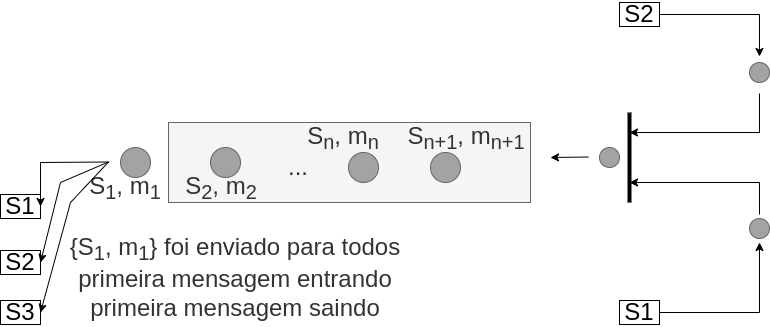
\includegraphics[width=0.8\linewidth]{figures/fifo.drawio.png}
    {\flushleft Fonte - Própria}
    \label{fig:fifo}
\end{figure}

A Figura \ref{fig:fifo} representa uma ideia de como o esquema de ordenação de mensagens FIFO pode funcionar. A ilustração em si demonstra que existe uma fila, que deve ser implementada por um ordenador de mensagens, assim as mensagens podem ser enfileiradas, ao passo que são enfileiradas, as mensagens também são consumidas na saída, dando vazão para as mensagens.

%\textbf{Causal}
\subsection{Ordem Causal}

A ordem causal, definida por Lamport \cite{lamport1978time}, estabelece algumas premissas: O símbolo $m$ é uma mensagem qualquer que acompanha um ID único e ${m_1, m_2, \dots, m_n} \in M$, onde M é um universo de mensagens; $send(m)$ é uma primitiva que executa o envio da mensagem $m \in M$; $p, q, r \in {participantes}$ onde os participantes são as entidades do sistema, que podem trocar mensagens entre si; $deliver(m)$ é uma primitiva de entrega de mensagens.

Na ordem causal, existe a definição da propriedade \textit{acontece antes}, simbolizado por $\longrightarrow$ e é um operador que designa uma ordem de precedência entre as mensagens.

Por ordem lógica, define-se: Uma mensagem $m_1$ precede logicamente $m_2$ \textit{i.e.} $m_1 \longrightarrow m_2$, sse: $m_1$ é enviada antes de $m_2$ pelo mesmo participante \textbf{ou} $m_1$ é entregue para o \textit{enviador} de $m_2$ antes que ele envie $m_2$ \textbf{ou} existe um $m_3$ tal que $m_1$ $\longrightarrow$ $m_3$ e $m_3$ $\longrightarrow$ $m_2$ \cite{PauloVerissimoLuisRodrigues}.
% Além disso,
%segue um paradigma lógico e é definida por \textcite{PauloVerissimoLuisRodrigues} como: ``

\textit{Exemplificando:} Se um evento $a$ aconteceu antes do evento $b$ \textit{i.e.} $a$ $\longrightarrow$ $b$, então o evento $b$ pode ter sido causado ou influenciado pelo evento $a$. Se $a$ e $b$ são duas mensagens \textit{multicast} (respeitando a causalidade), tem-se que a entrega de $a$ deve preceder a entrega de $b$, em todos os destinos comuns de $a$ e $b$. Abaixo está a especificação de entrega de pedido causal em grupos sobrepostos \cite{de1995causal}.

\begin{quote}
\textit{Definição de Ordem Causal}:\\
$send_p(m_1) \longrightarrow send_q(m_2)$
então
\\
$deliver_r(m_1) \longrightarrow deliver_r(m_2)$, \textit{i.e.} $m_1$
\\
é entregue para $r$ antes de $m_2$
\end{quote}

% Resumidamente, para quaisquer 
%2
% mensagens $m_1$ e, $m_2$ enviadas por $p$, respondidas por $q$, para o mesmo participante destinatário $r$, se $send_p(m_1) \longrightarrow send_q(m_2)$ então $deliver_r(m_1) \longrightarrow deliver_r(m_2)$, \textit{i.e.} $m_1$ é entregue para $r$ antes de $m_2$.
%'' 
A ordem causal pode ser implementada usando relógios lógicos de Lamport \cite{lamport1978time}
%, 
para capturar o sentido de causalidade sobre as entregas de mensagens.
%, entre os participantes. 
%A ordem causal permite eventos concorrentes acontecerem sem ordenamento, permitindo que computação paralela progrida sem restrições desnecessárias, mas em alguns casos é vital para o sistema que os eventos sejam ordenados \cite{PauloVerissimoLuisRodrigues}.

% Causal order lets concurrent events happen without ordering them. This is usually a positive feature, because it allows parallel computations to progress without unnecessary constraints.

\begin{figure}[htb!]
\centering
\caption{Exemplos de ordem causal}
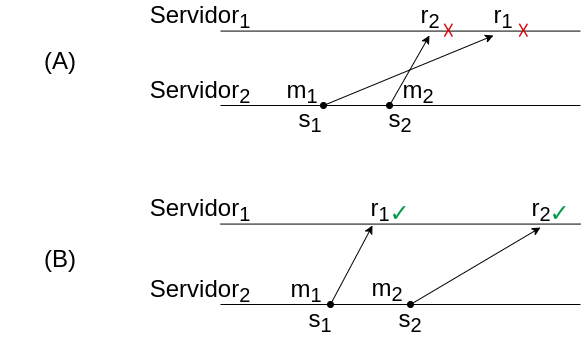
\includegraphics[width=0.8\linewidth]{figures/causal-order-works.drawio.png}
{\flushleft Fonte - Adaptado de \textcite{PauloVerissimoLuisRodrigues}}
\label{fig:causal-order-works}
\end{figure}

A Figura \ref{fig:causal-order-works} mostra dois exemplos (A e B) de ordem causal, os símbolos podem ser lidos da seguinte forma: $m_1$ e $m_2$ são mensagens, $s_1$ e $s_2$ são envios das mensagens, $r_1$ e $r_2$ são recebimentos das mensagens, $Servidor_1$ e $Servidor_2$ são os servidores do sistema distribuído. O exemplo (A) viola a ordem causal pois a mensagem $m_2$ chegou antes de $m_1$, sendo que $Servidor_2$ enviou primeiro $m_1$ e depois enviou $m_2$, ou seja, $m_1$ deve acontecer antes de $m_2$, pois existe uma relação de causa e ordem que deve ser obedecida. Essa relação pode ser observada no exemplo (B).

\subsection{Ordem Total}

Na ordenação total todos os participantes recebem as mensagens enviadas na mesma ordem. Porém, em termos mais técnicos, pode-se definir a partir de \textcite{PauloVerissimoLuisRodrigues} que:

\begin{quote}
\textit{Quaisquer duas mensagens entregues para quaisquer dois pares de participantes são entregues na mesma ordem para ambos os participantes.}
\end{quote}

O termo difusão em ordem total é também conhecido como difusão atômica, algumas vezes representado pela sigla \gls{AB-cast}. A seguir são apresentada as propriedades necessárias para assegurar ordenação total e os algoritmos para implementação de protocolo AB-cast.

% \begin{figure}[htb!]
%     \centering
%     \caption{Ilustração da ordenação total}
%     \includegraphics{figures/ordenacao-total.png}
%     \label{fig:total-ordering}
%     {\flushleft Fonte - Adaptado de \cite{journals/csur/DefagoSU04}}
% \end{figure}

% A Figura \ref{fig:total-ordering} ilustra o funcionamento da ordenação total, é possível observar que todas as mensagens que chegam, são difundidas de forma total e na mesma ordem de chegada.

%\subsection{Protocolos para Implementação de Ordem Total}
\section{Protocolos para Implementação de Ordem Total}

Define-se o problema com basicamente 2 primitivas e o conceito de processos corretos. As primitivas são \textit{TO-broadcast(m)} e \textit{TO-deliver(m)}, onde $m \in M$ é alguma mensagem que pode ser unicamente identificada e, que carrega a identificação do remetente, denotada por \textit{sender(m)} \cite{PauloVerissimoLuisRodrigues}.

A primitiva \textit{TO-broadcast} expressa a execução de difusão de uma mensagem para todos os processos corretos de um sistema, ou seja, todos esses processos corretos recebem as mesmas mensagens e na mesma ordem. \textit{TO-deliver} é outra primitiva que é executada sempre após \textit{TO-broadcast} \cite{PauloVerissimoLuisRodrigues}.

Os processos corretos pertencem a uma categoria de processos que não falham no sistema. Por exemplo, são processos que não omitem ou param de performar suas atividades de envio e recebimento de mensagens.
%, que respondem no tempo certo (exceto em sistemas assíncronos) e, que toleram falhas Bizantinas \cite{PauloVerissimoLuisRodrigues}. 
% A seguir é explanado alguns algoritmos que implementam \textit{TO-broadcast(m)}.

% qualquer outro algoritmo de consenso que utiliza ordem total como forma principal método de ordenação de mensagens.

A especificação básica para ordenação total,
conforme descrito por
%foi proposta por
\textcite{hadzilacos-10.5555/866693},
é apresentada a seguir:
%seguinte forma:

% \cite{journals/csur/DefagoSU04}
% (VALIDITY) If a correct process TO-
% broadcasts a message m, then it
% eventually TO-delivers m.

% (UNIFORM AGREEMENT) If a process TO-
% delivers a message m, then all correct
% processes eventually TO-deliver m.

% (UNIFORM INTEGRITY) For any message m,
% every process TO-delivers m at most
% once, and only if m was previously TO-
% broadcast by sender(m).

% (UNIFORM TOTAL ORDER) If processes p and
% q both TO-deliver messages m and m',
% then p TO-delivers m before m', if and
% only if q TO-delivers m before m'.

\begin{itemize}
\item \textbf{Validade}: Se um processo correto executa \textit{TO-broadcast} sobre uma mensagem $m$, então vai eventualmente executar \textit{TO-deliver} para a mensagem $m$.
\item \textbf{Acordo Uniforme}: Se um processo executa \textit{TO-deliver} sobre uma mensagem $m$, então todos os processos corretos irão eventualmente executar \textit{TO-deliver} sobre $m$.
\item \textbf{Integridade Uniforme}: Para qualquer mensagem $m$, cada processo executa \textit{TO-deliver} sobre uma mensagem $m$, pelo menos 1 vez, e apenas se previamente fora executado \textit{TO-broadcast} sobre uma mensagem $m$ por \textit{sender(m)}.
\item \textbf{Ordem Total Uniforme}: Se ambos os processos $p$ e $q$ executarem \textit{TO-deliver} sobre a mensagens $m$ e $m^{'}$, então $p$ executa \textit{TO-deliver} sobre $m$ antes de $m^{'}$, sse $q$ executa \textit{TO-deliver} sobre $m$ antes de $m^{'}$.
\end{itemize}

\subsection{Ordenação por sequenciador}

O algoritmo de ordenação por sequenciador tem a incumbência de ordenar todas as mensagens, sendo que para cada mensagem é associado um número de sequência. O algoritmo tem 3 papéis: o remetente (Algoritmo \ref{algo:simple-fixed-sequencer-sender}), o sequenciador (Algoritmo \ref{algo:simple-fixed-sequencer}) e os destinatários (Algoritmo \ref{algo:simple-fixed-sequencer-destinations}).

% \begin{enumerate}
% \item Todos os emissores enviam suas mensagens para o sequenciador.
% \item O sequenciador atribui um número de sequência único a cada mensagem.
% \item O sequenciador retransmite para todos os destinatários, usando ordem total.
% \end{enumerate}

%Logo a seguir expomos o algoritmo sequenciador fixo e, simples.

% \odo{O Algoritmo \ref{algo:simple-fixed-dest} apresenta .... } \ct{Indicar explicitamente e dizer o que cada algoritmo apresenta.}

% \textbf{Remetente}
% \begin{itemize}
% \item Executa a primitiva \textit{TO-broadcast(m)}, enviando \textit{send(m)} para o sequenciador.
% \end{itemize}

% \textbf{Sequenciador}
% \begin{itemize}
% \item Inicializa-se o número de sequência em 1.
% \item Quando o sequenciador recebe uma mensagem $m$
% \item O número de envio é inicializado com o valor de número de sequencia.
% \item Após isso, executa-se \textit{send(m, número de envio)} para todos os destinatários.
% \item Incrementa-se o número de sequência.
% \end{itemize}

% \textbf{Destinatários}
% \begin{itemize}
% \item Inicializa-se o número de próxima entrega em 1, e o conjunto de pendentes como vazio.
% \item Quando um processo destinatário recebe uma mensagem m com um número de sequência único.
% \item A mensagem m e, o número de sequência é unido ao conjunto de pendentes.
% \item Após unir as mensagens pendentes, executa-se um laço que percorre todas as mensagens que existem no conjunto de mensagens pendentes. Para cada $m$ que pertence ao conjunto de mensagens pendentes, executa-se \textit{entregar(m)}, ao final, incrementa-se o contador de próxima entrega.
% \end{itemize}

\begin{algorithm}
\DontPrintSemicolon
\procedure{TO-broadcast(m)} {
    send(m) to sequencer
}
\caption{Código dos remetentes para o algoritmo de sequenciador fixo simples}
\label{algo:simple-fixed-sequencer-sender}
\end{algorithm}


O Algoritmo \ref{algo:simple-fixed-sequencer-sender} apresenta a chamada do procedimento TO-broadcast(m). A primitiva TO-broadcast(m) é a representação da difusão por ordem total. Dentro do escopo do procedimento se executa a primitiva \textit{send(m)} ao sequenciador, discutido a seguir.

\begin{algorithm}
\DontPrintSemicolon

$seqnum := 1$

\when{receive(m)} {
    $sn(m) := seqnum$

    send(m, sn(m)) to all

    $seqnum := seqnum + 1$
}

\caption{Código do sequenciador para o algoritmo de sequenciador fixo simples}
\label{algo:simple-fixed-sequencer}
\end{algorithm}


O Algoritmo \ref{algo:simple-fixed-sequencer} representa o tratamento constante que é dado para mensagens $m$ que estão sendo recebidas. Começa com o número de sequência que recebe valor 1, esse valor é configurado uma vez apenas. Depois disto, o algoritmo só trata quando a mensagem $m$ existe e é recebida pela primitiva \textit{receive}.
O escopo de \textit{when receive(m)} tem 3 atribuições: na linha 3 o número de sequência de $m$ recebe o valor de \textit{seqnum} atual; na linha acontece o envio da mensagem $m$ junto com seu número de sequência através da primitiva \textit{send(m, sn(m))} para todos os participantes; na linha 5 ocorre o incremente do número de sequência.

\begin{algorithm}
\DontPrintSemicolon
\KwIn{Código do processo $p_i$}

${{nextdeliver}_p}_{i} := 1$\;
${{pending}_p}_{i} := \emptyset$\;

\when { receive (m, seqnum) } {
  ${{pending}_p}_{i} := {{pending}_p}_{i} \cup \{(m, seqnum)\}$\;
  \while { $\exists ({m}^{\prime}, {seqnum}^{\prime}) \in {{pending}_p}_{i}$ s.t. $seqnum^\prime = {{nextdeliver}_{p}}_{i}$} {
    \text{deliver}(${m}^{\prime}$)\;
    ${{nextdeliver}_p}_{i} := {{nextdeliver}_p}_{i} + 1$\;
  }
}
\caption{Código dos destinatários para o algoritmo de sequenciador fixo simples
\cite{journals/csur/DefagoSU04}}
\label{algo:simple-fixed-sequencer-destinations}
\end{algorithm}


O Algoritmo \ref{algo:simple-fixed-sequencer-destinations} inicializa os conjuntos de dados: \textit{nextdeliver} com todos os valores igual à 1, e \textit{ending} como vazio. Por conseguinte o algoritmo começa a processar continuamente o recebimento de mensagens, sendo que cada mensagem vem acompanhada de seu \textit{seqnum} (número de sequência). O primeiro passo dentro do escopo do \textit{when}, linha 4, implementa a união de novas mensagens no conjunto \textit{pending}. Quando o fluxo atinge a linha 5, ocorre um laço repetitivo. Neste laço repetitivo se verifica a existência de uma mensagem $m$ com \textit{seqnum} pertencente ao conjunto \textit{pending}, se for o caso então \textit{seqnum} receberá o valor de \textit{nextdeliver[$p_{i}$]} (final da linha 5). Após isso duas linhas de código são executadas, na linha 6 ocorre a execução da primitiva \textit{deliver(m)}. E na linha 7, ocorre o incremento de \textit{nextdeliver} na posição de $p_{i}$.


% \begin{comment}
% \odo{
% Exemplo de algoritmo. O Algoritmo \ref{alg:t} é apenas um exemplo de algoritmo em LaTeX, caso seja útil para você.

% \begin{algorithm}[!htb]

% %\caption{Transaction}\label{alg:t}
% \caption{T($cid,t$)}\label{alg:t}
% \begin{algorithmic}[1]
%   \State $ws \leftarrow \varnothing$; $rs \leftarrow \varnothing$; $i \leftarrow 0$;
%   \State choose randomly one of the replica servers $s$ \label{code:select_server}
%   %\ForAll {$t.getOp(i)$} \label{code:ws1}
%   \While {$t.getOp(i) \neq commit \wedge t.getOp(i) \neq abort$} \label{code:ws1}
%     \If {$t.getOp(i) = write$} \label{code:ws2}
%       \State $ws \leftarrow ws \cup (t.getItem(i),t.getValue(i))$
%     \EndIf
%     \If {$t.getOp(i) = read$}	
%       \If {$t.getItem(i) \in ws$}  \label{code:ws_copy1}
%         \State return $v$, s.t. $(t.getItem(i),v) \in ws$ \label{code:ws_copy2}
%       \Else
%         \State $c2s[s]!read,t.getItem(i),cid$  \label{code:read_request1}
%         \State $s2c[cid]?v,version$ from $s$  \label{code:read_request2}
%         \State $rs \leftarrow rs \cup (t.getItem(i),v,version)$ \label{code:read_request3}
%       \EndIf
%     \EndIf
%     \State $i$++;
%   \EndWhile
%   \If {$t.getOp(i) = commit$}   \label{code:if_commit}
%       \State $abcast.send(com\_req,cid,t.id,rs,ws)$    \label{code:abcast}
%       \State $s2c[cid]?outcome,s$	%\Comment{receive the $outcome$ from $s$}          
%       \State $t.result = outcome$ 
%   \Else \label{code:if_abort}
%       \State $t.result = abort$ 
%       %\State $return$ 
%   \EndIf

% \end{algorithmic}
% \end{algorithm}
% }
% \end{comment}

\subsection{Ordenação baseada em privilégio}

O algoritmo baseado em privilégio tem 2 papéis principais: os remetentes (Algoritmo \ref{algo:priviledge-based-simple-senders}) e os destinatários (Algoritmo \ref{algo:priviledge-based-simple-destinations}). A intenção geral do algoritmo é implementar a difusão atômica, para isso, rotaciona-se um \textit{token} entre os remetentes. Quando cada remetente recebe o \textit{token}, na sua vez, executa-se a primitiva \textit{tosend}, enviando para todos os destinatários as mesmas mensagens e na mesma ordem de chegada.
% Uma desvantagem do algoritmo baseado em privilégio é a dificuldade em atingir bons níveis de justiça (\textit{fairness}) entre todos os remetentes, a seguir exibimos o algoritmos remetentes e destinatários respectivamente.

% \textbf{Remetentes}

% \begin{itemize}
% \item Os enviadores são dispostos na forma de uma fila giratória (ou fila anelar).
% \item O primeiro da fila recebe o índice 0, e assim sucessivamente.
% \item A fila então deverá girar, porém quem começa operando é o $\text{sender}_0$.
% \item Quando a fila circula, o token deve ser passado ao próximo \textit{sender}.
% \item É atribuído para cada envio de mensagem um \textit{token} com número de sequência único.
% \item O procedimento de \textit{enviar} é basicamente \textit{TO-broadcast(m)}. Como já vimos, \textit{TO-broadcast(m)} é uma primitiva que faz a difusão ordem total das mensagens para os demais participantes do sistema.
% \item Quando um remetente recebe um \textit{token}, executa-se o seguinte: para cada destinatário \textit{send(m, número de sequencia do token)}, após isso, incrementa-se número de sequência do \textit{token}.
% \item Esse remetente passa o \textit{token} para o próximo da fila giratória.
% \item Como incrementamos o número de sequência do \textit{token}, não haverá colisão de número de sequências, e as mensagens poderão ser unicamente identificadas pelo seu número de sequência, no momento que o \textit{token} foi passado adiante.
% \end{itemize}

% \textbf{Destinatários}

% O algoritmo dos destinatários para o algoritmo baseado em privilégio é equivalente ao código para destinatários do algoritmo sequenciador fixo e simples.

\pagebreak

\begin{algorithm}
\DontPrintSemicolon
\KwIn{Código do processo $s_i$}

${{tosend}_s}_{i} := \emptyset$\;

\If {$s_i = s_1$} {
  token.seqnum := 1\;
  send token to $s_1$\;
}

\procedure { TO-broadcast(m) } {
  ${{tosend}_s}_{i} \cup \{m\}$\;
}

\when {receive token} {
  \foreach { ${m}{\prime}$ in ${{tosend}_s}_{i}$ } {
    send(${m}^{\prime}$, token.seqnum) to destinations\;
    $\text{token.seqnum} := \text{token.seqnum} + 1$\;
  }
  ${{tosend}_s}_{i} := \emptyset$\;
  send token to ${s}_{i+1 \mod n}$
}
\caption{Código dos remetentes para o algoritmo baseado em privilégios}
\label{algo:priviledge-based-simple-senders}
\end{algorithm}


O Algoritmo \ref{algo:priviledge-based-simple-senders} inicializa o conjunto \textit{tosend} como vazio. Se o processo $s_i$ é o primeiro, então inicializa \textit{token.seqnum} com 1 (linha 3) e, executa-se a primitiva \textit{send(token)} para $s_1$. Na linha 5 executa-se o procedimento de difusão ordem total sobre a mensagem $m$, na linha 6 a mensagem $m$ é unida ao conjunto \textit{tosend}. Na linha 7 quando o código dos remetentes recebe um novo token, executa-se, na linha 8, um laço iterativo, ou seja, para cada $m$ dentro do conjunto \textit{tosend}, executa-se, na linha 9, a primitiva \textit{send} para a mensagem $m$ junto com o valor atual de token.seqnum (rotacionando) para os destinatários. Na linha 10 a variável \textit{token.seqnum} recebe um incremento de 1. Fora do laço repetitivo, na linha 11, o conjunto \textit{tosend} recebe vazio. Na linha 12 executa-se a primitiva \textit{send} sobre o objeto \textit{token} para o processo $s$ porém é feito um cálculo modular para iterar pelos processos participantes de forma anelar. Uma vez que o próximo processo obtêm o \textit{token}, é a vez do processo recebedor de executar o algoritmo.

\begin{algorithm}
\DontPrintSemicolon
\KwIn{Código do processo $p_i$}

${{nextdeliver}_p}_{i} := 1$\;
${{pending}_p}_{i} := \emptyset$\;

\when { receive (m, seqnum) } {
  ${{pending}_p}_{i} := {{pending}_p}_{i} \cup \{(m, seqnum)\}$\;
  \while { $\exists ({m}^{\prime}, {seqnum}^{\prime}) \in {{pending}_p}_{i}$ s.t. $seqnum^\prime = {{nextdeliver}_{p}}_{i}$} {
    \text{deliver} ${m}^{\prime}$\;
    ${{nextdeliver}_p}_{i} := {{nextdeliver}_p}_{i} + 1$\;
  }
}
\caption{Código dos destinatários para o algoritmo baseado em privilégios \cite{journals/csur/DefagoSU04}}
\label{algo:priviledge-based-simple-destinations}
\end{algorithm}


O Algoritmo \ref{algo:priviledge-based-simple-destinations} e o Algoritmo \ref{algo:simple-fixed-sequencer-destinations} são iguais e portanto têm as mesmas explicações.

\section{Consenso}
\label{sec:consenso}

Protocolos de consenso distribuído também podem ser utilizados para implementar entrega totalmente ordenada de requisições \cite{conf/dsn/EkwallS06, MilosevicHutleSchiper2011}. Esses protocolos surgem como uma boa alternativa, visto que a difusão atômica pode gerar uma quantidade muito grande de requisições. Segundo \textcite{lamport2001paxos}, os algoritmos de consenso precisam garantir 3 premissas básicas:

\begin{itemize}
\item \textbf{Não trivialidade}: Um valor é aprendido se e somente se tiver sido proposto e aceito pela maioria dos participantes.

\item \textbf{Estabilidade}: A cada rodada de aprendizagem, qualquer processo participante deve aprender no máximo um valor. Um valor aprendido não deve ser alterado posteriormente pois um valor aprendido será executado na aplicação.

\item \textbf{Consistência}: A cada rodada de aprendizagem, dois processos diferentes não devem aprender valores diferentes.
\end{itemize}

\subsection{Protocolos de Consenso}

Protocolos de consenso são centrais para a implementação de aplicações distribuídas tolerantes a falhas \cite{cason2017role}.
O problema de consenso surgiu da necessidade de múltiplos
%computadores que compartilham o estado do sistema, 
processos chegarem a um acordo sobre um determinado valor. 
%Ou seja, para atingirmos harmonia entre os 
Portanto, participantes de um sistema distribuído
%de computadores precisamos de
necessitam de
um algoritmo capaz de estabelecer 
%um inquérito entre as máquinas. 
um quórum decisivo sobre um valor proposto pelo algoritmo de consenso.
%Veja que até o momento não precisamos mencionar se existe um tipo de aplicação específica, pois esse consenso é algo anterior a isso e, que deve estabelecer um acordo sobre algum comando antes desse comando ser executado por uma determinada aplicação.

% A seguir são apresentados 
%duas tecnologias, 
% dois protocolos de consenso
% bastante conhecidos
%, 
% na literatura.
%e, que implementam consenso, tipicamente ambos tem a intenção de oferecer uma evolução gradual e baseada em máquina de estados, da replicação dos \textit{logs} internos que contêm comandos que irão alterar o estado interno de uma aplicação.

\subsubsection{Paxos}

O algoritmo Paxos foi desenvolvido por \textcite{lamport2001paxos} e geralmente se implementa Paxos entre um conjunto distribuído de computadores trocando mensagens de forma assíncrona. Por exemplo, um cliente envia um valor ao sistema e o protocolo Paxos é invocado para propor este valor aos participantes. Quando a maioria dos participantes que executam o Paxos concordarem sobre o valor proposto, então este valor será aprendido e entregue aos interessados neste valor, por exemplo, a um conjunto de réplicas. Existem 3 papéis no algoritmo Paxos:

\begin{itemize}
\item \textit{Proponente:} Recebe solicitações de valores externos e as propõem aos aceitadores. Cada proposta nova deve conter um número único identificador e maior que a proposta anterior.

\item \textit{Aceitadores:} Aceitam determinado valor proposto pelo proponente e informam ao proponente e aos aprendizes se algum valor foi aceito. Uma resposta de um aceitador representa um voto para uma proposta. 
\item \textit{Aprendizes:} Aprendem o resultado do consenso, se houver.
\end{itemize}

\begin{figure}[htb!]
\centering
\caption{Exemplo de troca de mensagens no protocolo Paxos}
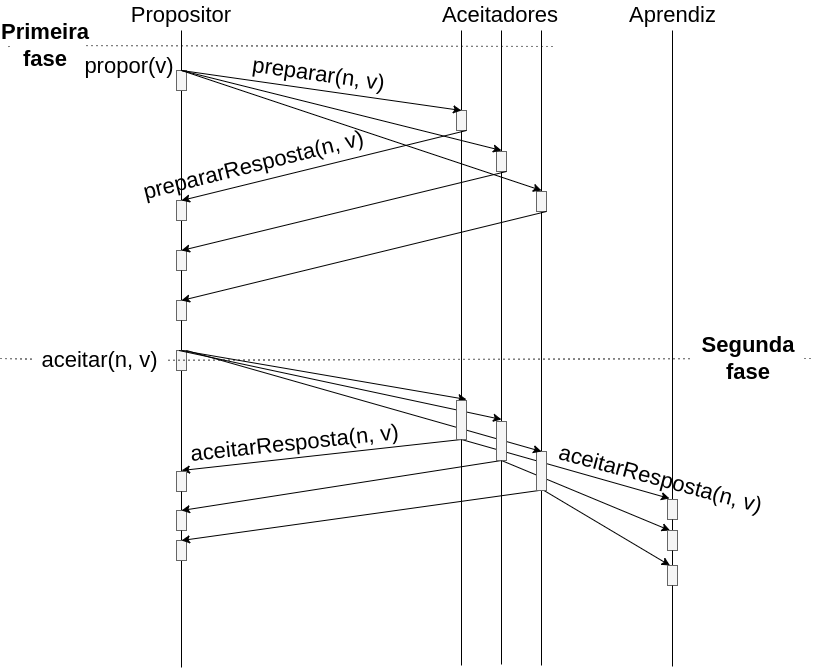
\includegraphics[width=1\linewidth]{figures/paxos.png}
{\flushleft Fonte - Adaptado de \textcite{AcaciaTerra}}
\label{fig:protocolo:paxos}
\end{figure}

O Paxos tem basicamente duas fases e a Figura \ref{fig:protocolo:paxos} ilustra as fases 1ª e 2ª. As fases foram subdivididas em a-b e que serão brevemente discutidas, a seguir.

\begin{enumerate}

\item \textit{Primeira fase: Proposta e Preparação}

\begin{enumerate}
\item O protocolo se inicia quando um proponente recebe um valor $v$. O valor $v$ pode ser, por exemplo, um comando que será executado em um determinado momento (no caso a natureza do valor $v$ depende muito da aplicação \textit{stateful}). O proponente propõe um valor $v$ enviando uma mensagem igual para cada um dos aceitadores. O algoritmo envia uma mensagem $v$ por proposta e está proposta terá outra difusão de mensagens para cada um dos aceitadores. Cada mensagem contém o valor da proposta e um número de sequência. O número de sequência é um identificador da proposta e quando o propositor propõe um valor $v$, este também prepara as mensagens e envia aos aceitadores.

\item Os aceitadores avaliam a proposta de valor e emitem suas respostas ao propositor, sinalizando que reconheceram a mensagem $m$ (que acompanha um número de sequência como identificador, juntamente com o valor proposto). Os aceitadores só devem aceitar a proposta com o número de sequência maior do que qualquer outro. A proposta já aceita com número identificador menor que o atual serão descartadas.
\end{enumerate}

\item \textit{Segunda fase: Aceitação e Aprendizado}

\begin{enumerate}

\item Os aceitadores recebem uma segunda rodada de mensagens,\\
onde o propositor
envia as mensagens, nesse estágio o propositor envia uma sequência de mensagens
para aceitar o valor $v$ com o número de sequência $n$, ou seja, os aceitadores 
recebem\\ \textit{aceitar(n, v)}.

\item O aprendiz aprende se os aceitadores chegaram a um consenso em uma rodada específica do algoritmo. A quantidade de aceitadores precisa ser pelo menos metade mais um, do conjunto de servidores do sistema. Se a maioria dos aceitadores responderem que concordam com o valor $v$, então $v$ será aprendido.
\end{enumerate}
\end{enumerate}

\pagebreak

\subsubsection{Raft}

O Raft é um algoritmo distribuído e assíncrono de ordenação de eventos \cite{raft}. Este algorítimo espera que exista um sistema de replicação de \textit{logs} em cada instância que executa o protocolo, e cada instância do sistema Raft pode estar em um dos seguintes estados: Líder, Candidato, Seguidor, porém só existe um líder por vez e o líder recebe requisições do cliente e pode propor mensagens aos seguidores.

\begin{figure}[htb!]
\centering
\caption{Fases de um serviço Raft}
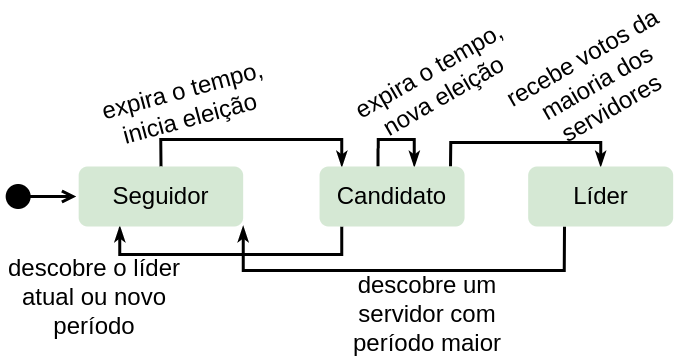
\includegraphics[width=0.75\linewidth]{figures/raft-states.drawio.png}
\label{fig:raft}
{\flushleft Fonte - Adaptado de \cite{raft}}
\end{figure}

A Figura \ref{fig:raft} ilustra os estados de cada nó participante e as possíveis transições. Os seguidores reagem às propostas do líder. Se os candidatos não recebem mais sinais do líder, elege-se um novo líder dentre os candidatos. Se algum candidato estiver no estado de seguidor, este deve poder votar por propostas que chegam ou votar para a eleição de novos líderes. É responsabilidade do líder fazer a replicação dos \textit{logs}. Deve haver apenas 1 líder por termo. O líder é responsável pela replicação de \textit{logs}.

\textcite{raft} buscaram desenvolver o algoritmo Raft com técnicas que aumentassem a legibilidade do algoritmo. Algumas das técnicas utilizadas foram: decomposição do problema em pequenas partes, minimização do espaço de estados, tratar múltiplos problemas com um único mecanismo, eliminação de casos especiais e minimização de não-determinismo.

% \item Os autores do Raft desenvolveram um mecanismo para decidir sobre informações obsoletas. Esse mecanismo se chama \textit{Term}.
% \item A ordem de prioridade dos termos aumentam de acordo com qual termo é mais recente. Os termos mais recentes são mais importantes. Existe então alguma noção de tempo inserida no algoritmo Raft.

\begin{figure}[htb!]
\centering
\caption{Termos em Raft}
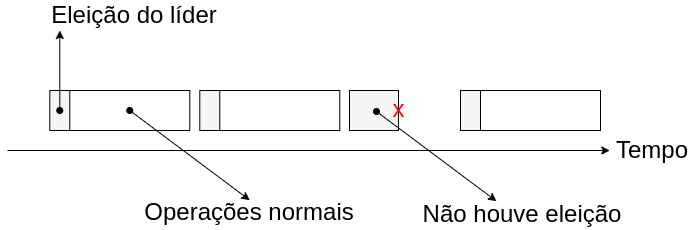
\includegraphics[width=0.8\linewidth]{figures/terms-raft.drawio.png}
{\flushleft Fonte - Adaptado de \textcite{raft}}
\label{fig:terms-raft}
\end{figure}

A Figura \ref{fig:terms-raft} ilustra um exemplo do funcionamento dos termos em Raft. Os \textit{Termos} em Raft existem para que o Raft possa identificar informação obsoleta e distinguir de informação nova. Cada máquina do \textit{cluster} mantêm o seu \textit{termo} atual e não são compartilhados globalmente. Cada \textit{Termo} se trata de um período de tempo onde ocorre uma eleição de um líder e após isso ocorrem proposta. Um \textit{Termo} é subdividido em 2 fases:

\textit{Primeira fase:} será feita a escolha de um líder.

\textit{Segunda fase:} serão feitas propostas de mensagens aos seguidores.

% Alguns \textit{Termos) podem não ter líder presente, quer dizer que houve falha na eleição.

% \subsubsection{Comparação entre Raft e Paxos}

% Em termos de provas formais, ambos buscam formalizar em provas matemáticas e premissas imutáveis, basicamente 4 regras formais dão embasamento formal. As regras formais são propriedades para atingir consenso assíncrono entre as partes envolvidas. A partir de estudos posteriores, os autores \textcite{MOSTEFAOUI_RAYNAL} esmiuçaram 4 regras formais e, que hoje estão elucidadas nas premissas a seguir:

% The Consensus Problem
% In the Consensus problem, every correct process Pi proposes a value v\ and all
% correct processes have to decide on the same value v, that has to be one of the
% proposed values. More precisely, the Consensus problem is defined by three safety
% properties (Validity, Integrity and Uniform Agreement) and a Termination Property
% [4,10]:
% [4] Chandra T. and Toueg S., Unreliable Failure Detectors for Reliable Distributed Systems. Journal of the ACM, 43(2):225-267, March 1996
% [10] Fischer M.J., Lynch N. and Paterson M.S., Impossibility of Distributed Consensus with One Faulty Process. Journal of the ACM, 32(2):374-382, April 1985
% • Validity: If a process decides v, then v was proposed by some process.
% • Integrity: A process decides at most once.
% • Uniform Agreement: No two processes decide differently.
% • Termination: Every correct process eventually decides on some value.

% \begin{enumerate}
% \item Validade: apenas os valores propostos podem ser decididos. Se um processo decidir sobre um valor, v, então algum processo precisa ter proposto v.
% \item Acordo uniforme: dois processos corretos (aqueles que não falham), não podem decidir sobre valores diferentes.
% \item Integridade: cada processo pode decidir 1 valor pelo menos 1 vez.
% \item Termo: todos os processos vão, eventualmente, decidir sobre um resultado.
% \end{enumerate}

% O Kubernetes, por padrão, não permite que StatefulSets obedeçam a terceira regra, Integridade. Apenas o nó mestre pode escrever na aplicação stateful, e se o nó mestre falhar outro nó deve ser eleito mestre, do contrário o cluster não irá mudar.

% Em termos de sistemas distribuídos, ambos servem casos de uso semelhantes, por exemplo: ``Quando múltiplas réplicas chegam à uma conclusão sobre um único comando?''. Paxos generalmente sacrifica disponibilidade \cite{cason2017role}, e o Raft opera as custas de disponibilidade. Quando nos deparados com particionamento de redes, Paxos vai continuar disponível, mas o \textit{cluster} Raft pode ficar parcialmente indisponível. Raft, e Paxos, são algoritmos de consenso que confiam na maioria do \textit{cluster}, em constante comunicação, para evoluir de estado. Em termos de didática, Raft tem um propósito de ser fácil de se compreender, enquanto Paxos não tem essa premissa. Ambos Paxos e Raft vão continuar operando enquanto o \textit{cluster} enfrenta falhas em seus nós.










% \section{Replicação por Máquinas de Estados}
% \label{sec:rep_maq_est}

% Implementar Replicação por Máquina de Estados (\gls{RME}) fornece tolerância a falhas. Também fornece escalabilidade, pois os clientes podem ler dados de qualquer servidor disponível
% \cite{lamport1978implementation, schneider1990}. 
% %O uso de Replicação por Máquina de Estados 
% %\odo{(\gls{RME})}
% %(RMS) 
% %foi proposto por \textcite{schneider1990} e, é comumente discutida na literatura o uso de RMS baseada em \textit{logs} \cite{lamport2001paxos}. 
% %Uma vantagem de usarmos máquina de estado é a promoção de tolerância a falhas e, o aumento da disponibilidade do sistema \cite{lamport1978implementation, schneider1990}. 
% De maneira geral, para a replicação por máquinas de estados funciona da seguinte forma: Configuramos um \textit{cluster} com várias máquinas replicando um mesmo serviço (\textit{i.e.} Banco de dados), e a medida que os clientes fazem suas requisições, a máquina de estados age como um replicador de \textit{logs}. Uma pré-condição para que todas as réplicas de máquina de estado se comportem de forma idêntica é executar as mesmas entradas de comando na mesma ordem. Os \textit{logs} aqui são as instruções que vão alterar dados da aplicação que o \textit{cluster} está servindo \cite{PauloVerissimoLuisRodrigues}. Os autores \cite{AlbuquerqueAlchieriCaetanoSolis2018} contribuíram com algumas especificações para Replicação por Máquina de Estados. A seguir será mostrado duas opções de modelagem, para manter serviços replicados:

% \begin{itemize}
% \item Apenas 1 mestre fixo que recebe todas as solicitações, e repassa essas solicitações para os demais participantes do sistema.
% \item Qualquer réplica pode se tornar um mestre eventualmente, através de um algoritmo de eleição.
% \end{itemize}

% Existem duas primitivas envolvidas em RME:

% \begin{enumerate}
% \item \textit{invoke(operation)}: essa primitiva é executada pelos clientes para chamar operações no serviço que implementa RME.
% \item \textit{execute(operation)}: essa primitiva é executada pelos servidores replicados, sempre que uma operação deve ser executada pelo serviço de RME.
% \end{enumerate}

% Além disso existem algumas propriedades para tornar o RME determinístico.

% \begin{itemize}
% \item Estado inicial: todas as réplicas corretas devem inciar a partir de um mesmo estado.
% \item Determinismo: todas as réplicas corretas, que executam uma mesma operação sobre um mesmo estado, realizam a mesma mudança em seus estados e produzem a mesma resposta.
% \item Coordenação: todas as réplicas corretas executam a mesma sequência de operações.
% \end{itemize}

% % \subsection{Replicação Ativa}

% % Difusão atômica é uma primitiva que tem influência quando se implementa replicação ativa \cite{lamport1978implementation, schneider1990}. A replicação ativa é uma técnica intuitiva que pode ser aplicada a máquinas de estado. Consiste em ter várias réplicas da mesma máquina de estado executadas por diferentes processos. Para garantir que o estado dessas réplicas seja mantido consistente, um protocolo de ordenação total deve ser usado para difundir os comandos da máquina de estado, no caso do \cite{PauloVerissimoLuisRodrigues}.

% A máquina de estados deve estar presente em cada réplica, e compartilhar um \textit{log} em comum e, a ideia é executar comandos do \textit{log}, igualmente em cada réplica, como é possível ver na Figura \ref{fig:rms}. Os comandos do \textit{logs} são comandos que foram autorizados por um algoritmo de consenso.

% \begin{figure}[htb!]
% \centering
% \caption{Eventos da Replicação por Máquinas de Estados}
% 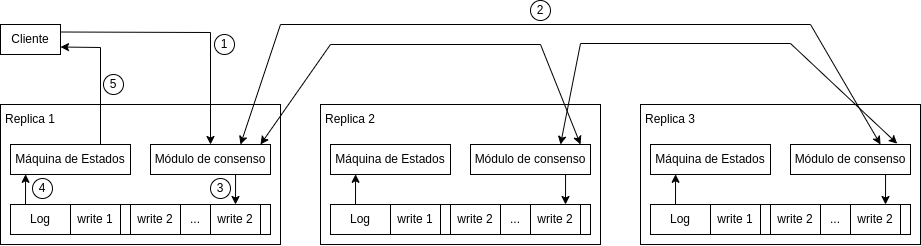
\includegraphics[width=1\linewidth]{figures/rms.drawio.png}
% {\flushleft Fonte - Adaptado de \textcite[p.~233]{journals/dbsk/SkrzypzcakS20}}
% \label{fig:rms}
% \end{figure}

% A Figura \ref{fig:rms} mostra que em um sistema distribuído essa máquina de estados deve ser replicada, ou seja, todos os servidores deste sistema distribuído deverão executar a mesma máquina de estados. Para fins de explicação, estamos considerando o módulo de consenso como uma caixa preta. As marcações numeradas na Figura \ref{fig:rms} são respectivamente:

% \begin{enumerate}
% \item Envia um comando qualquer para a Máquina de Estados Replicada.
% \item Entre em consenso sobre o comando.
% \item Concatena o novo comando.
% \item Aplica o comando que está na fila para ser executado, e que está no \textit{log}.
% \item Responde ao cliente.
% \end{enumerate}

% Cada nó, de um sistema distribuído, pode ser pensado como uma máquina de estados determinística. O intuito é prover tolerância a falhas, executando o mesmo registro de comandos, após cada ponto de salvamento. Idealmente essa é a ideia básica, porém na realidade existem  complicações, essas complicações motivam a pesquisa e desenvolvimento desse trabalho acadêmico. A imagem a seguir exemplifica, de maneira abstrata, como seria a replicação máquina de estados paralela. O desafio aqui é replicar o registro de comandos, igualmente, para todas as máquinas do sistema. Depois da replicação feita é necessário impor uma sincronização para que eles executem os comandos e a aplicação \textit{stateful} transite de estado, gerando um novo estado, porém são várias aplicações replicadas e iguais ao final do processo.










\section{Arquitetura de microsserviços}
\label{sec:arq_micro}

Publicações recentes mostram que implementar em arquiteturas de microsserviços provê desacoplamento e escalabilidade \cite{carrasco2018migrating, bavskarada2018architecting, zdun2019emerging}. O trabalho de \textcite{fritzsch2018monolith} provê dez abordagens estratégicas de refatoração, viabilizando migrar monólitos para microsserviços. A implementação de software seguindo arquitetura de microsserviços requer desenvolvimento de partes modulares, onde cada módulo pode ser conectado e desconectado em outros sistemas, sem que haja necessidade de mudar o sistema principal que faz uso do microsserviço. Geralmente, os microsserviços são enxutos com \textit{interfaces} específicas que viabilizam extensibilidade de funcionalidades específicas \cite{journals/software/JamshidiPMLT18}.

% não tenho citações pra isso
% Desenvolver arquitetura de microsserviços em Kubernetes tornou-se vigente, partindo do princípio de um \textit{cluster} servindo uma aplicação replicada. O \textit{cluster} Kubernetes permite que os desenvolvedores abstraiam a funcionalidade de um conjunto de \textit{Pods} e a exponham a outros desenvolvedores por meio de uma \gls{API}\footnote{API ou \textit{Application Programming Interface} é um conjunto de rotinas e padrões que facilitam a comunicação e troca de mensagens entre sistemas.}

% \subsection{Contêiner}

% A tecnologia de contêiner segue a característica de isolar várias tecnologias dentro de um pacote, os contêineres são diferentes de máquinas virtuais, por causa do advento em Linux de cgroups e namespaces, pois permitem que os contêineres usufruam diretamente dos recursos físicos, da máquina alvo.

\subsection{Contêineres e Orquestradores de contêineres}

% \textbf{O que é}

Um contêiner se trata de um ambiente empacotado de: software, configurações, dependências além de outras coisas para tornar possível que um serviço seja executado isoladamente de outros softwares da máquina hospedeira.

Um orquestrador é um gestor de contêineres com características de auto-cura e elasticidade. Também pode ser usado para a criação de \textit{cluster} (conjunto de máquinas interligadas por uma rede). Dependendo do fabricante da tecnologia algumas características podem mudar, porém geralmente o orquestrador tem características de: escalonamento de réplicas baseado em métricas, balanceamento de carga. Orquestradores podem operar sob os contêineres em grupos específicos \cite{casalicchio2019container}, descomplicando de se aplicar atribuições específicas para cada grupo de contêineres e podendo-se criar divisões lógicas que aprimoram a especificação do \textit{cluster} como um todo.

% \textbf{Contêineres}

\subsection{Docker}

Um contêiner Docker\footnote{\url{https://github.com/docker}} \cite{docker/docs/2022} é uma instância executável de uma imagem. Uma imagem do Docker é um modelo \textit{read only} que provê instruções para construção de um contêiner Docker. O Docker é uma tecnologia de código-aberto que oferece: preparo, entrega e execução de aplicativos auto-contidos em contêineres. Com Docker é possível: criar, iniciar, parar, mover e excluir um contêiner usando a \gls{API} do Docker. O Docker integra com funcionalidades Linux como \textit{cgroups} e \textit{namespaces} para usufruir dos recursos da máquina hospedeira, permitindo melhor desempenho. Além disso, existe uma extensa comunidade adepta ao Docker, que contribui com melhorias constantes ao Docker. 

% Existem várias alternativas ao Docker, alguns exemplos são: Podman, LXD, Containerd. Para este trabalho, optou-se pelo Docker pois existe uma documentação extensa e, muitos contribuidores, por exemplo desenvolvedores implementam soluções e as compartilham no DockerHub (uma central de implantações prontas). O Docker também é bastante aceito pela comunidade científica para aumento da reprodutibilidade \cite{CitoGallDockerReproducibility}. Além disso nem todas as tecnologias de contêiner são suportados pelo Kubernetes.

% \textbf{Por quê usamos Kubernetes}

% Segundo \textcite{soppelsa2016native} existem alternativas ao Kubernetes, por exemplo o Docker Swarm. Swarm é um modo nativo da tecnologia Docker, que permite orquestração dos contêineres, ou seja herda as características de auto-cura, balanceamento de carga, \textit{etc}. Kubernetes da suporte para Docker, Containerd, CRI-O e, qualquer outra tecnologia de contêiner que implementa a interface Kubernetes CRI (Container Runtime Interface) \cite{kubernetes/docs/2022}, e uma vantagem de usarmos Kubernetes é devido ao Kubernetes CRI. O Docker Swarm poderia ser usado no lugar de Kubernetes, porém estamos enxergando muito mais aderência ao Kubernetes do que outras alternativas, nas bases científicas, um dos motivos pode ser a influência da Google sob o Kubernetes, apesar de hoje em dia não ser mais um projeto Google, mas sim um projeto da \textit{Cloud Native Computing Foundation}. Esperamos saber responder como Kubernetes se comporta após ter sido incrementado com serviço de replicação por máquinas de estados e consenso, ou seja, quais são as vantagens e desvantagens.

\subsection{Kubernetes}

Kubernetes é uma ferramenta de orquestração de contêineres inicialmente desenvolvida por engenheiros da Google. Kubernetes providencia primitivas tais como: Nodes, Services, Pods, Deployment, Job, Secret, ReplicaSet, StatefulSet, Volume, dentre outras, para que desenvolvedores possam definir Clusters. Kubernetes resolve problemas de estabelecimento de rede entre as máquinas que compõe o Cluster, sejam elas físicas ou virtuais. Kubernetes também resolve problema de replicação de serviços, todavia não garante que os dados das réplicas serão replicados de maneira consistente \cite{kubernetes/docs/2022}. Quando se trata de sistemas com replicação, busca-se uma infraestrutura robusta que permite que cada réplica possa ter seus recursos garantidos \cite{Stubbs2015DistributedSO}, baseado em métricas e tolerante a falhas \cite{vayghan2021kubernetes}.

\subsubsection{Detalhes da tecnologia Kubernetes}

A disponibilidade do Kubernetes foi avaliada por \cite{vayghan2021kubernetes} e o Kubernetes provê mecanismos que operam para deixar o Cluster operacional e servindo. A escalabilidade e recuperação de desastres é algo que o Kubernetes prove automatizações pré-configuráveis. A escalabilidade permite expandir ou retrair a quantidade de nós de trabalho no \textit{cluster}, dependendo da carga sob demanda. A recuperação de desastres trata de prover a restauração de \textit{Pods} em casos de falhas. Dentre os vários tipos de componentes do Kubernetes se pode mencionar alguns básicos:

\textit{Nodes:} São máquinas físicas ou virtuais que têm como principal função executar os \textit{Pods}. Tipicamente um nó em Kubernetes é visto como um servidor. A infraestrutura do Kubernetes segue o esquema Líder-Seguidores, onde o nó líder opera sob os nós seguidores.

\textit{Services:} Um \textit{Service} define um conjunto de \textit{Pods} que provê serviços variados.

% Uma vez que o \textit{cluster} Kubernetes está configurado, será necessário o uso de um outro componente interno chamado Kubernetes DNS (\textit{Domain Name System}). O Kubernetes provê um serviço de DNS capaz de localizar os endereços dos \textit{Pods}, no \textit{cluster}. O DNS \textit{server} do \textit{cluster} Kubernetes é instalado no sistema quando o \textit{cluster} é criado no sistema operacional \textit{host}. A função do Kubernetes DNS é fornecer a localização em termos do IP de cada nó do \textit{cluster}.

% Kubernetes:Pod

\textit{Pod:} A menor unidade que o orquestrador administra, um \textit{Pod} pode conter múltiplos contêineres em execução, mas tipicamente cada \textit{Pod} contém apenas uma aplicação isolada em contêiner. \textit{Pod} são efêmeros, significa que podem encerrar seu ciclo de vida, se um \textit{Pod} morrer um novo \textit{Pod} será alocado no lugar. Cada \textit{Pod} recebe um endereço IP\footnote{IP: \textit{Internet Protocol} se trata de um endereço que identifica um dispositivo na rede.} mas se um \textit{Pod} morrer e for substituído por um novo, o endereço IP permanece o mesmo.

% Kubernetes:Kubectl

\textit{Kubectl:} É uma ferramenta de comandos em linha, para ser executado em um \textit{Terminal}. O Kubectl permite executar operações em Kubernetes, mas é preciso um arquivo \textit{YAML} que descreve tudo sobre o \textit{cluster} Kubernetes.

% Kubernetes:PersistentVolumes

\textit{PersistentVolumes:} Se trata de um componente que administra a persistência dos dados, podendo ser local ou remoto. O Kubernetes não faz backup dos dados, ficando a cargo do desenvolvedor implementa-lo. Os modos de acesso aos volumes persistentes são: leitura e escrita por um nó único (\gls{RWO}); somente leitura por vários nós (\gls{ROX}); leitura escrita por vários nós (\gls{RWX}).

% O \textit{Pod} com permissão de escrita dos dados é chamado de \textit{leader}, os demais \textit{pods} são chamados de \textit{followers}. Uma vez que novos dados foram escritos no banco, um outro mecanismo fará a sincronização dos dados, fazendo com que todos as aplicações \textit{stateful} evoluam igualmente. Para manter os dados preservados é necessário configurar \textit{PersistentVolume} para \textit{StatefulSet}, pois os ciclos de vida do \textit{PersistentVolume} e do \textit{StatefulSet} são desacoplados. Cada \textit{Pod} em modo \textit{StatefulSet} recebe um nome especial no formato de \textit{\$\{statefulset name\}-\$inteiro positivo começando de 0}. O Kubernetes não faz a clonagem, sincronização ou, o \textit{backup} dos dados, ficando a cargo do desenvolvedor configurar isso dentro do \textit{StatefulSet}.

% O \textit{Heartbeat} é um sinal que o nó seguidor emite para o nó mestre avisando qual o estado de saúde dos \textit{Pods}.

% O Kubernetes provê um componente de armazenamento chave-valor e não-volátil, chamado Etcd. O banco Etcd funciona como o cérebro do Kubernetes. O Etcd armazena dados de todos os nós, assim o Kubernetes pode executar ações de \textit{auto medicação}, ou \textit{auto escalonamento}, baseando-se nas informações sobre os estados de cada \textit{Pod} do \textit{cluster} Kubernetes.

% Kubernetes:{Kubelet, ApiServer, PodSpec, YAML}

\textit{Kubelet:} É um componente básico de cada um Nó do Kubernetes. O \textit{Kubelet} é requisitado pelo Kubernetes do nó controlador para receber informações sobre estatísticas de todos os nós do cluster, com essas essas informações o Kubernetes faz a gestão automática dos Nós e seus componentes internos.

% Kubernetes:ReplicaSet

\textit{ReplicaSet:} Mantêm as réplicas de um \textit{cluster} Kubernetes. É definido com os campos: seletor que especifica como identificar os \textit{Pods}, número de réplicas indicando quantos \textit{Pods}, e um \textit{template} do \textit{Pod} para poder replicar igualmente.

\textit{Deployment:} O Deployment define como criar e atualizar instâncias do seu aplicativo.

% Kubernetes:LoadBalancer

% Para podermos manter o balanceamento de carga do \textit{cluster}, Kubernetes provê um componente chamado \textit{LoadBalancer}, que direciona as requisições para réplicas. Métricas como quantidade de: UCP disponível, Memória Ram, Latência da rede, \textit{etc}., podem ser usadas para definir qual replica receberá a carga de trabalho.

% Balanceamento de carga funciona de forma diferente para aplicações Stateful

% Kubernetes:Secrets

% É importante também lembrar de manter em segredo algumas informações sensíveis. O Kubernetes \textit{Secrets} é outro componente do Kubernetes que guarda as informações sigilosas, da sua aplicação tais como senhas, \gls{API} \textit{tokens}, \textit{ids}, etc., sem que os desenvolvedores precisem ter isso no código da aplicação ou nos arquivos de configuração. É necessário que os dados sigilosos guardados no \textit{Secrets} estejam codificados em base64. No entanto o \textit{Secrets} não encripta os dados sigilosos, por padrão. O desenvolvedor precisa seguir alguns passos para ter os dados criptografados no \textit{Secrets}.

\textit{Jobs}: é um componente que pode criar um ou mais \textit{Pods}, e executará um procedimento até que os \textit{Jobs} possam terminar. O Kubernetes mantém o número de Jobs que estão finalizando com sucesso e, se esse número chegar até um valor especificado então o Kubernetes vai entender como missão bem sucedida.

% \begin{figure}[!htb]
% \centering
% \caption{Arquitetura do \textit{Cluster} Kubernetes}
% 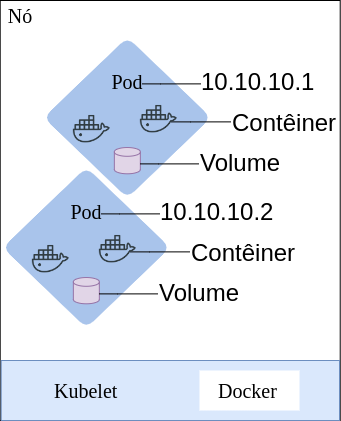
\includegraphics[width=0.4\linewidth]{figures/kubernetes-arch.png}
% {\flushleft Fonte - Adaptado de \textcite{renan2021hermes}}
% \label{fig:kubernetes-architecture}
% \end{figure}

% A Figura \ref{fig:kubernetes-architecture} representa uma forma de esquematizar um \textit{cluster} Kubernetes com o Hermes servindo à frente de uma aplicação \textit{stateful} alvo. O \textit{cluster} Kubernetes pode conter vários nós, cada nó tem 1 Kubelet e suporte para Docker contêineres, cada nó pode conter 1 ou mais \textit{Pods}, cada \textit{Pod} tem 2 imagens de contêineres (uma para o Hermes e outra para a aplicação \textit{stateful} alvo, cada \textit{Pod} tem seu IP na rede privada do Kubernetes e cada Pod contêm seu volume persistente. O padrão de projeto Sidecar, foi implementado junto ao Kubernetes, onde o contêiner do Hermes é lançado ao lado do contêiner da aplicação alvo.

% ---

% ---
% 3 - Capítulo 3
% ---
\chapter{Trabalhos Correlatos}
\label{cap:correlatos}

A seguir alguns trabalhos relacionados a ordenação de mensagens em arquiteturas de microsserviços e abordagens em orquestração de contêineres. A pesquisa por trabalhos publicados foi feita de maneira exploratória, visando bases científicas tais como: \gls{ACM}, \gls{IEEE}, \gls{SBC}, dentre outras.

\section{Relacionados a implementação de arquitetura de microsserviços}

Trabalhos recentes na literatura têm apresentado diversas soluções envolvendo ordenação de mensagens em arquitetura de microsserviços. Os benefícios de arquiteturas de microsserviços abrangem: modularidade e escalabilidade.

% É comum encontrarmos trabalhos que utilizam a técnica de replicação por máquina de estado, onde um conjunto de máquinas devem manter sincronia, evoluindo igualmente, apesar das falhas que pode ocorrer no sistema, um exemplo é uma das máquinas parar de responder e ser declarada como inalcançável.

\subsection{A Kubernetes controller for managing the availability of elastic microservice based stateful applications}

Segundo \textcite{vayghan2021kubernetes} a arquitetura de microsserviços vêm ganhando muita popularidade. A arquitetura de microsserviços faz a junção de módulos fracamente acoplados, que podem ser escalados independentemente. Esse trabalho avalia o uso de microsserviços em contêineres orquestrados por Kubernetes, mas o Kubernetes recebeu um incremento de software que visa controlar os estados de alta disponibilidade dos contêineres. Nesse trabalho de \textcite{vayghan2021kubernetes} foram identificados arquiteturas para implantar aplicações em microsserviços com Kubernetes. Esse trabalho também realizou experimentações com o Kubernetes da perspectiva de sua capacidade de disponibilidade. Os resultados dos experimentos mostraram que as ações de reparo do Kubernetes não puderam satisfazer alguns limites de alta disponibilidade, avaliados. Em outros casos o Kubernetes não pode garantir recuperação do serviço. Os autores propuseram um controlador de estados de alta disponibilidade integrado ao Kubernetes, que permite replicação de estados de aplicação e redirecionamento automático de serviço. As avaliações foram feitas sob as perspectivas de disponibilidade e escalabilidade. Os resultados das investigações mostram que a solução pode melhorar o tempo de recuperação de aplicações \textit{stateful} baseadas em microsserviços, em 50\%.

% \subsection{COMO O TRABALHO DESENVOLVEU A SOLUÇÃO}

\textcite{vayghan2021kubernetes}
%buscaram endereçar problemas como disponibilidade e tolerância a falhas. Mas como fizeram isso? Eles(as) 
implementaram uma ferramenta
%que vamos descrever um pouco a seguir. A solução deles(as) integra o conceito de Estados de Alta Disponibilidade (do Inglês, \textit{HA states}) (exemplos: quando ativo; quando esperando) com o Kubernetes. Assim eles buscaram aumentar a disponibilidade de aplicações baseadas
para alta disponibilidade 
em arquiteturas de microsserviços em \textit{clusters} Kubernetes. O fizeram por recuperar o estado do serviço depois que o \textit{Pod} do Kubernetes foi reparado. Agregaram ao Kubernetes um novo componente chamado Controlador de Estados de Alta Disponibilidade (do Inglês, \textit{High Avaliability State Controller}, abreviado como SC).
% \subsection{COMO OBTIVERAM RESULTADOS (ALTO NÍVEL)}
Conduziram um conjunto de experimentos em arquiteturas de microsserviços em um sistema distribuído físico.
% Pelo artigo é possível notar que houve muito estudo sobre o funcionamento de \textit{StatefulSets} em Kubernetes.
Para cada arquitetura experimentada pelo trabalho, o número de \textit{Pods} implantados é igual a 10 (dez). Em cada conjunto de experimentos se encerra o contêiner da aplicação dos K \textit{Pods} ativos, onde K são inteiros de 1 até 5. Os outros \textit{Pods} ficam vivos para serem avaliados (discutidos em seguida). Em cada rodada dos experimentos são feitas medições de \textit{disponibilidade}, para cada \textit{Pod} que tenha falhado.

Além disso, são comparados com as falhas simultâneas de múltiplos \textit{Pods} afetam métricas de disponibilidade. Medições de disponibilidade são as métricas que avaliam a disponibilidade do serviço de cada \textit{Pod}. As medições na experimentação medem o tempo de reação, tempo de reparo, tempo de restauração e tempo total de indisponibilidade. Tempo de total de indisponibilidade é um período quando a energia suprida ou outro serviço não está mais disponível ou quando um equipamento é encerrado por alguma razão. Outra medição feita nos experimentos é de tempo de escalonamento e se trata da latência desde o momento de envio das requisições, para escalar máquinas, até o momento do último \textit{Pod} implantado.

% \begin{figure}[ht!]
% \centering
% \caption{Funcionamento em alto nível do Controlador de estados de alta disponibilidade (versão adaptada)}
% \centering
% \includegraphics[width=0.6\linewidth]{capitulos/simplificacao-kubernetes.png}
% \caption{fonte: Adaptação de \textcite{vayghan2021kubernetes}.}
% \end{figure}

% \subsection{AS LIMITAÇÕES DA ABORDAGENS DO TRABALHO}

Uma possível limitação é que o software implementado deve ser compreendido para poder ser utilizado. Um desenvolvedor deverá buscar o Kubernetes modificado ao invés do original e terá que compreender a implementação feita por \textcite{vayghan2021kubernetes}.

% \subsection{RELAÇÃO DESSE TRABALHO COM O NOSSO}

\textcite{vayghan2021kubernetes} fez contribuições em algoritmos, ou seja programação de software que agrega funcionalidades novas ao Kubernetes. Outra forma de contribuição é como interceptar a \textit{API} do Kubernetes, ou seja, como observar os eventos. Outros benefícios desse artigo são maneiras de configurar o Kubernetes para prover replicação das instâncias da aplicação. Finalmente, se relaciona com o presente trabalho por estas contribuições mencionadas e nas questões de avaliação do sistema em arquiteturas de microsserviços, dando importância também para escalabilidade.

% Além disso esse trabalho nos ensina como construir experimentações e avaliações da solução, usando uma metodologia de perguntas e respostas.

%%%%%%%%%%%%%%%%%%%%%%%%%%%%%%%%%%%%%

\subsection{\textit{Incorporating the Raft consensus protocol in containers managed by Kubernetes: an evaluation}}

O trabalho de \textcite{netto2020incorporating} visa implementar uma solução de replicação por máquinas de estados usando Raft como algoritmo de consenso. A sua solução foi construída no topo do orquestrador de contêineres Kubernetes. Esse trabalho optou por utilizar o Raft ao invés do Paxos, pela didática e praticidade.

Para desenvolver a solução os autores escolheram o algoritmo Raft e buscaram um código livre e aberto em linguagem Go. O código foi inserido no contexto de orquestração de contêineres. Esse trabalho visou utilizar o banco de dados Etcd\footnote{\url{https://etcd.io/} para fins práticos e demonstrativos da solução}. Os autores estenderam uma biblioteca para poder acrescentar funcionalidades personalizadas ao Kubernetes. Foram adicionados:

\begin{itemize}
\item Mecanismo próprio de descoberta de réplicas usando API do Kubernetes.
\item Aceitação de requisições por qualquer réplica.
\end{itemize}

% No trabalho os contêineres incluem processos para comunicar com a API do Kubernetes. Através dessa comunicação, cada contêiner periodicamente pergunta sobre os endereços IP de outras réplicas.
% O Kubernetes permite que todas os pods recebam requisições.

A implementação de \textcite{netto2020incorporating} permite que as réplicas líder possam receber requisições e assim é possível redirecionar as requisições para o líder. Se o líder falhar outras réplicas podem executar o papel de líder.

% \subsection{COMO OBTIVERAM RESULTADOS (ALTO NÍVEL)}

Eles criaram um ambiente de experimentação real, para experimentações diversas. Eles organizaram o sistema distribuído físico para que atendessem as necessidades da pesquisa. Os autores compararam 3 cenários, sendo eles:

\begin{itemize}
\item A implementação KRaft
\item A implementação Raft (exclusivo ao Etcd\footnote{O Etcd é banco de armazenamento chave-valor distribuído usado para armazenar e gerenciar as informações críticas que os sistemas distribuídos precisam para continuar funcionando.}, embutido no Kubernetes)
\item Um sistema não replicado.
\end{itemize}

O número de clientes fazendo requisições simultâneas aos servidores variou de 4 até 64 para fins de experimentação. Para fazer medições constantes em cada instância os autores usaram um software Linux chamado \textit{dstat}. Os resultados desse trabalho focam bastante em latência (em ms) e vazão (em requisições por segundo). Houveram testes com várias quantidades de clientes acessando a plataforma Kubernetes, e além disso foi comparado a solução KRaft, com Raft, e sistema não replicado.

% \subsection{AS LIMITAÇÕES DA ABORDAGENS DO TRABALHO}

Alguns dos resultados do artigo mostraram que a latência por tempo foi menor do que o sistema replicado, e não há aprofundamento sobre as causas. Outros resultados apontaram que a solução se mostrou limitada na questão de vazão de requisições por tempo. Já outros resultados mostraram análises dos consumos de recursos, a saber, Memória e CPU. Porém não se demonstrou o quanto as máquinas físicas e o Kubernetes consomem de Memória e, CPU. Não foi possível identificar, com clareza, as comparações entre a solução e o Raft do Kubernetes.
% Em um outro resultado os autores comparam volumes de dados enviados pela rede (em MB/s), mas segundo eles mesmos os resultados foram equivalentes, o que causa dúvida.

% \subsection{RELAÇÃO DESSE TRABALHO COM O NOSSO}

O trabalho em questão é ortogonal ao presente trabalho pelos aspectos de métricas de experimentação, latência e vazão. Construção de um ambiente de experimentação físico. Uso de protocolo de consenso visando implementar ordenação de mensagens com algoritmos de consenso. Abordagens em arquiteturas de microsserviços. Uso de Kubernetes para orquestrar contêineres. Isolamento de aspectos de implementação em contêineres.
% E finalmente, avaliação do consumo de recursos.


%%%%%%%%%%%%%%%%%%%%%%%%%%%%%%%%%%%%%

\pagebreak

\subsection{\textit{Implementação de um interceptador para ordenação de mensagens em arquiteturas baseadas em microsserviços}}

\textcite{renan2021hermes} propôs uma arquitetura em ambientes de microsserviços para o desacoplamento da lógica de ordenação de mensagens. Um dos objetivos era manter consistência forte em um sistema replicado. Para isto, implementou-se replicação por máquinas de estados usando intercepção de mensagens que chegam ao serviço Hermes. O serviço, baseia-se em padrões de projeto voltados para arquiteturas de microsserviços. O código criado por \textcite{renan2021hermes} provê interfaces que uma vez implementadas possibilitam que outros protocolos de consenso sejam incluídos, e também outros protocolos de comunicação.

O \textit{Hermes} foi programado em linguagem Go\footnote{Golang: \url{https://go.dev/}}. O autor utilizou Kubernetes e Docker para criar o sistema de interceptação, pois cada instância do serviço sendo replicado tem uma outra instância do Hermes à frente, interceptando as requisições. Uma vez interceptadas, as mensagens são submetidas ao protocolo de consenso, para ordenação das mensagens. O \textit{Hermes} utiliza o algoritmo Raft para realizar a ordenação.

A avaliação da ferramenta aconteceu através de experimentação no Emulab \cite{emulab-10.1145/844128.844152}, um ambiente para criação de uma rede física de máquinas. O provisionamento do ambiente foi automatizado com a ferramenta Ansible\footnote{Ansible: \url{https://www.ansible.com/}}. Os cenários básicos de avaliação foram: sem replicação, replicação à nível de aplicação e replicação no interceptador.

As comparações mostram que o Hermes satura relativamente mais rápido que o caso sem replicação. Aparentemente os resultados nos mostram que a medida que a vazão média cresce, a latência (ms) tende a acompanhar, porém em alguns pontos a latência tem um comportamento inverso.

Alguns resultados mostraram uma vazão maior para o cenário de replicação a nível de aplicação. No entanto, para replicação a nível de interceptador mostraram uma vazão menor e em um outro resultado avaliando a latência, inverteram-se os papéis. Aparentemente existem limitações com relação a vazão.
% Houve pouca clareza em mostrar como as cargas de trabalho foram pensadas e trabalhadas até que os gráficos demonstrassem a curva de saturação.

% \subsection{RELAÇÃO DESSE TRABALHO COM O NOSSO}

A relevância deste trabalho está relacionada ao fato de o trabalho atual estar estendendo as funcionalidades do Hermes, para adicionar uma nova forma de comunicação. É notável o estudo aprofundado do código Hermes, bem como as técnicas, métodos, conceitos, algoritmos por trás do funcionamento do Hermes.

% \subsection{Relacionados a replicação com o uso de orquestrador de contêineres}

% \textcite{netto2020incorporating}
% \cite{netto2020incorporating}
% \parencite{netto2020incorporating}

% Estratégias de replicação por máquinas de estados não são novas para os pesquisadores. Trabalhos atuais têm demonstrado avaliações em ambientes reais, além de utilizar orquestradores de contêineres, (como Kubernetes ou outros), para poder gerir as réplicas distribuídas. Cada réplica serve uma aplicação que é construída em contêiner, em Docker ou outra  tecnologia. Os trabalhos de \textcite{netto2020incorporating} e \textcite{renan2021hermes} contribuem com estratégias de replicação por máquina de estados em arquitetura de microsserviços, aplicando em imagens Docker, orquestradas por Kubernetes. O trabalho de \textcite{vayghan2021kubernetes} não utiliza Raft como algoritmo de consenso entre réplicas, pois havia uma necessidade de entender os limites em replicação pelo Kubernetes ao utilizar o sistema próprio de \textit{StatefulSet}, por outro lado \textcite{netto2020incorporating} e \textcite{renan2021hermes} utilizaram Raft.

% https://kubernetes.io/docs/tasks/run-application/run-replicated-stateful-application/
% https://kubernetes.io/docs/tasks/run-application/run-replicated-stateful-application/
% https://kubernetes.io/docs/tasks/run-application/run-replicated-stateful-application/
% https://kubernetes.io/docs/tasks/run-application/run-replicated-stateful-application/

% \subsection{Relacionados ao uso de mensageiros para replicação}

% O trabalho de \textcite{Petrescu2020LogRI} propôs um sistema que visa utilizar o Apache Kafka, um sistema de troca de mensagens, com Raft, um algoritmo de consenso entre as réplicas. Esse trabalho propõe utilizar-se de um mecanismo próprio para troca de mensagens para transferir \textit{logs} de replicação entre as réplicas. Outro trabalho de \textcite{okusanya2019consensus}, também segue uma linha parecida usando Raft, porém se utiliza uma tecnologia diferente para troca de mensagens, o ZMQ Poller, um mecanismo de notificação e escuta, baseado em eventos, via sockets.


% ---

\chapter{Hermes}
\label{cap:hermes}

O Hermes \cite{renan2021hermes} é um interceptador de mensagens, entre o cliente e servidor. O Hermes é encarregado de ordenar as mensagens usando algoritmos de consenso. Após ordenadas as mensagens, o Hermes entrega as mensagens aos servidores replicados.

O objetivo do Hermes é abstrair os detalhes da ordenação de requisições em sistemas replicados em arquiteturas de microsserviços. Trata-se de um conjunto de interfaces que visam oferecer uma camada de abstração. O Hermes usa o padrão de projetos \textit{proxy}, uma vez que as requisições chegam até o Kubernetes, o serviço do Hermes as intercepta e faz o tratamento de obter consenso entre as réplicas. O cliente envia as requisições para o Hermes, mas isso fica transparente ao usuário. O módulo Hermes utiliza a biblioteca \textit{Hashicorp Raft}\footnote{Hashicorp Raft: \url{https://github.com/hashicorp/raft}}.

% \textbf{Hermes}

O Hermes tem propósitos de ser desacoplado, escalável e compartimentado em tecnologia de contêiner Docker e orquestrado em Kubernetes. Utilizar o Kubernetes é parte do mecanismo de interceptação e também serve para fazer gestão das réplicas. O sistema usufrui de mecanismos do Kubernetes que isolam as réplicas em seus \textit{Nodes} específicos:

\begin{itemize}
\item Afinidade e Anti-Afinidade: Forçar o Kubernetes a inserir uma réplica para cada nó, afastando-as em máquinas físicas, para que cada \textit{Pod} tenha seus recursos garantidos.
\item NodeSelector: localizar as réplicas de Hermes com o servidor alvo em Nós especificos com a label \textit{server}. Segregar os clientes dos servidores, em nós.
\end{itemize}

O interceptador Hermes utiliza padrões de projeto de microsserviços. Os padrões utilizados foram \textit{Proxy} \cite{chelliah2017architectural} e \textit{Sidecar} \cite{Sidecarp49:online}. O padrão \textit{Proxy} foi escolhido por fornecer meios lógicos para interceptar mensagens dos clientes e manter um distanciamento das regras de negócio do servidor alvo. O padrão Sidecar foi usado para separar as operações de ordenação de mensagens da aplicação por trás do Hermes, reduzindo sua complexidade interna e deixando a cargo do Hermes para fazer a ordenação de mensagens.

\pagebreak

\section{Hermes em arquitetura de orquestração de contêineres}

\begin{figure}[!htb]
\centering
\caption{Arquitetura do Hermes}
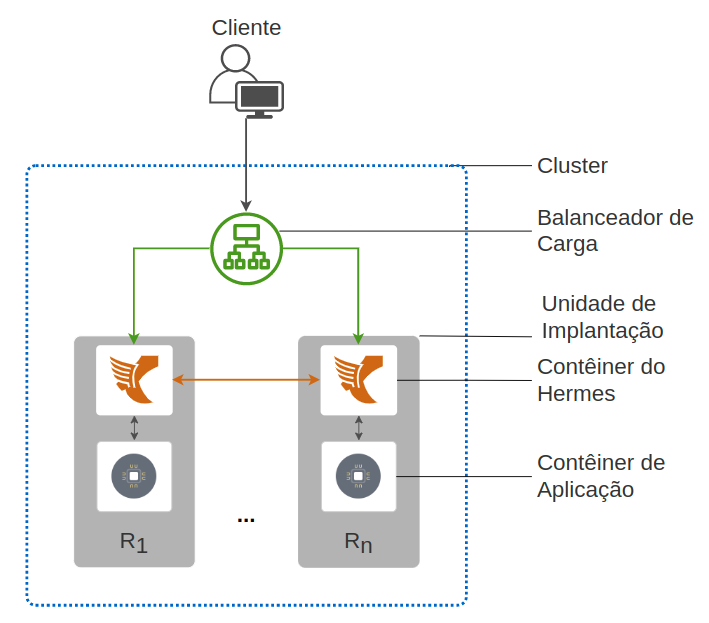
\includegraphics[width=0.8\linewidth]{figures/hermes-overview.png}
{\flushleft Fonte - \textcite{renan2021hermes}}
\label{fig:hermes-architecture}
\end{figure}

A Figura \ref{fig:hermes-architecture} mostra a arquitetura do Hermes em orquestrador de contêineres. O contêiner do Hermes se localiza à frente do contêiner de aplicação. O bloco cinza se trata da unidade de implantação, onde podem haver as unidades $R_{1}, R_{2}, R_{3}, \ldots, R_{n}$. A diferença é que quando o cliente envia uma mensagem qualquer para algum serviço, o balanceador de carga irá repassar essa mensagem para um Hermes, esse Hermes fará o papel de interceptar a mensagem e depois irá executar a ordenação de mensagens, uma vez ordenadas as mensagens o Hermes executa a aplicação dessas mensagens nos contêineres da aplicação. Desta maneira se implementa o padrão de projetos Sidecar, pois o Hermes está ao lado do contêiner de aplicação e a comunicação entre os contêineres de Implantação e de Aplicação é feita através de endereço \gls{IP} e porta.

% \textbf{Interface}

% \textbf{Padrão \textit{Interceptor}}

% \textbf{Onde o interceptador se encontra}

A aplicação está contida dentro dos \textit{Pods}, e cada \textit{Pod} tem um Hermes e uma aplicação alvo sendo replicada. As requisições chegam para o Hermes líder que repassa a mensagem em bytes para o Raft poder ordenar usando consenso entre os participantes.

% O Hermes, por sua vez, deve acionar o algoritmo de consenso para poder ordenar as mensagens recebidas. O banco de dados chave valor \textit{etcd} pode ser usado para armazenar informações essenciais para o funcionamento do algoritmo de consenso.

\section{Detalhes de implementação do Hermes}

O desenvolvimento sobre as classes de projeto do Hermes requer que alguns conceitos sejam observados.

\begin{figure}[!htb]
\centering
\caption{Relação entre os componentes do interceptador Hermes}
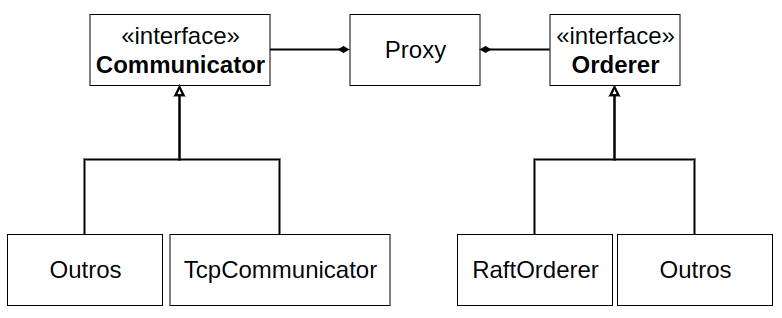
\includegraphics[width=0.9\linewidth]{figures/hermes-components.png}
\label{fig:componentes-hermes}
{\flushleft Fonte - Adaptado de \textcite{renan2021hermes}}
\end{figure}

A Figura \ref{fig:componentes-hermes} mostra a arquitetura do Hermes em UML. O Hermes foi implementado com padrão de projeto Proxy que por sua vez é composto de 2 objetos, sendo um \textit{comunicador} e um \textit{ordenador}. O \textit{comunicador} implementa a interface \textit{Communicator} e o ordenador implementa a interface \textit{Orderer}.

\begin{figure}[!htb]
\centering
\caption{Interfaces do código Hermes}
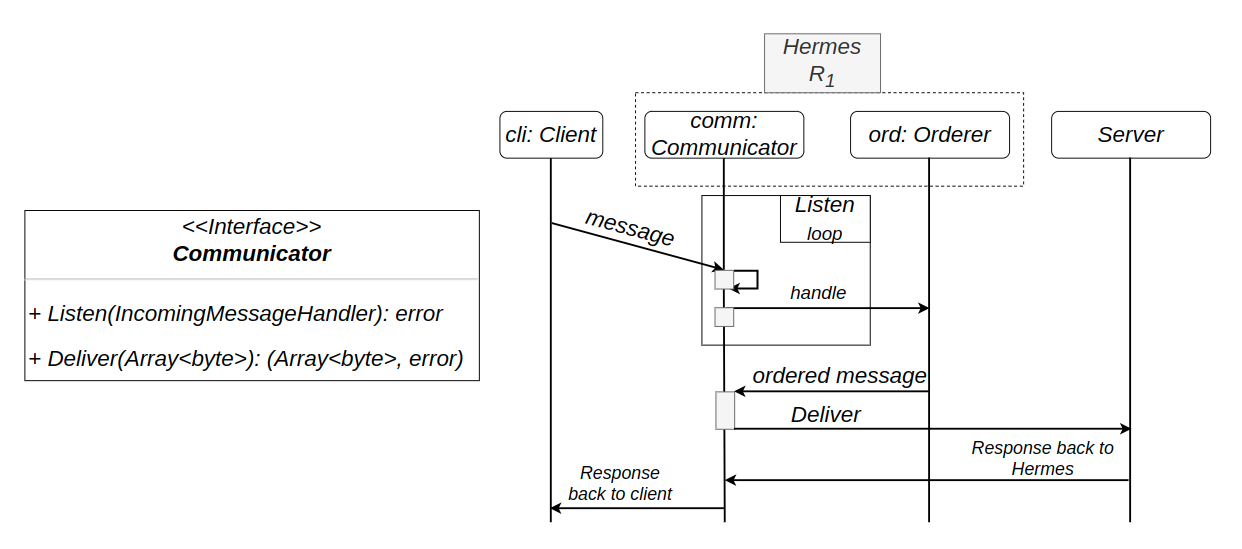
\includegraphics[width=\linewidth]{figures/communicator.drawio.png}
{\flushleft Fonte - Adaptado de \textcite{renan2021hermes}}
\label{fig:communicator-interfaces-hermes}
\end{figure}

A Figura \ref{fig:communicator-interfaces-hermes} mostra a interface \textit{Communicator} com os métodos \textit{Listen} e \textit{Deliver} ao lado de um diagrama de mensagens para ilustrar o funcionamento da interface. É possível observar que o método \textit{Listen} permanece escutando mensagens do \textit{Client}. Assim que uma mensagem é capturada, transforma-se esta mensagem para bytes e se envia para o \textit{Orderer}, através do método \textit{IncomingMessageHandler} que fora previamente configurada. A parte do \textit{Orderer} está omitida no diagrama, porém o \textit{Orderer} irá processar a mensagem, executando um algoritmo específico de ordenação de mensagens \textit{i.e.} Raft ou Paxos. Depois de ordenar a mensagem, o \textit{Orderer} retorna a mensagem em bytes para o método \textit{Deliver}, o \textit{Deliver} irá trabalhar a mensagem e finalmente envia para o servidor de aplicação, porém com a certeza que a mensagem já foi ordenada. Após isto o Hermes ainda pode receber uma resposta do Servidor replicado e assim o Hermes pode repassar a resposta para o \textit{Client}.

\begin{figure}[!htb]
\centering
\caption{Interfaces do código Hermes}
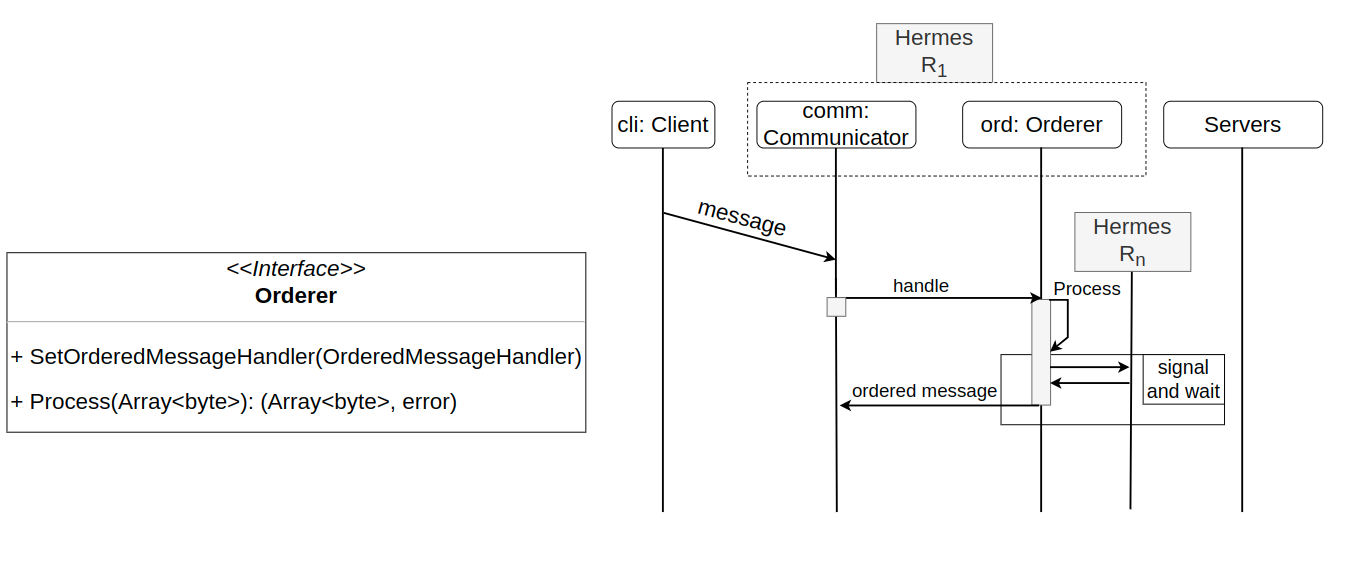
\includegraphics[width=\linewidth]{figures/orderer.drawio.png}
{\flushleft Fonte - Adaptado de \textcite{renan2021hermes}}
\label{fig:orderer-interfaces-hermes}
\end{figure}

A Figura \ref{fig:orderer-interfaces-hermes} mostra a interface \textit{Orderer} com os métodos \textit{SetOrdererMessageHandler} e \textit{Process} ao lado de um diagrama de mensagens para ilustrar o funcionamento da interface. Focando no \textit{Orderer}, assim que a mensagem chega para o \textit{Orderer} através do método IncomingMessageHandler, essa mensagem será executada pelo método Process que recebe uma mensagem em \textit{bytes}, depois de executar o algoritmo de ordenação e interagir com as outras réplicas de Hermes então será feita a aplicação da mensagem nos servidor de aplicação.


% ---
% 4 - Capítulo 4
% ---
\chapter{Implementação da interface de comunicação no Hermes}
\label{cap:http}

\section{Mudanças}

Foram realizadas mudanças no desenvolvimento na forma de comunicação do Hermes. A mudança permite, o Hermes aceitar requisições HTTP de maneira genérica. Para isso, foi necessário implementar a interface \textit{Communicator}. Durante o desenvolvimento, foi criado um projeto do Hermes com: Docker, Docker Compose e Delve\footnote{Delve é um depurador de código linguagem Go.}. A implementação tomou o nome de \textit{HttpCommunicator}, seguindo o padrão de nomes previamente implementado.

As requisições HTTP do tipo GET e POST podem ter uma resposta do servidor de aplicação. Esta resposta também foi considerada na implementação do HttpCommunicator, e uma vez que a requisição foi ordenada a requisição pode ser aplicada ao servidor alvo, uma vez que a resposta está pronta ela pode ser repassada ao cliente. O Hermes fará este serviço de ordenação de forma transparente ao usuário.

A intercepção é um trabalho de fatores em conjunto, começando pelo Kubernetes e os arquivos YAML que descrevem o \textit{cluster} Kubernetes. Os arquivos \textit{YAML} têm as descrições de Afinidades, Anti-Afinidades, e \textit{nodeSelector} para atrelar cada \textit{Pod} replicado ao seu nó servidor específico.

\subsection{Implementação}

A classe \textit{HTTPCommunicator} está localizada em \textit{pkg/communication/http.go}. Para implementar a \textit{HTTPCommunicator} foram usadas as bibliotecas \textit{net/http, bufio, bytes, io/ioutil}, dentre outras. A necessidade de estender as bibliotecas de conversão de bytes foi para poder transformar a requisição em bytes e enviar ao \textit{handler} ordenador de mensagens. Uma vez que o Hermes devolve a mensagem ordenada para o \textit{HTTPCommunicator}, é preciso transformar a mensagem de bytes para uma Requisição executável pela biblioteca \textit{net/http}.

\begin{minipage}{\textwidth}
\begin{center}
\lstinputlisting[language=Go, numbers=left, firstnumber=1, numberstyle=\scriptsize\color{black}, caption={Código na versão resumida do HttpCommunicator}, label={lst:codigo-httpcomm}]{chapters/algorithms/http.go}
\end{center}
\end{minipage}

O Algoritmo \ref{lst:codigo-httpcomm} pode ser entendido da seguinte forma: A linha 14 converte a requisição \gls{HTTP} para \textit{bytes} (código omitido). A linha 16 faz com que o Hermes acione o mecanismo de ordenação de mensagens, passando os bytes para serem ordenados. Depois que os bytes foram ordenados eles vão eventualmente retornar para o \textit{Deliver} para serem entregues para o servidor da aplicação, para isso a linha 2 converte os bytes em requisição (código omitido). Com a requisição convertida, altera-se o \textit{HOST} alvo nas linhas 4-6. A variável \textit{RequestURI} na linha 8 está sendo transformada para \textit{string} vazia, pois a biblioteca de \textit{net/http} proíbe que a mesma requisição seja usada, desta maneira a biblioteca aceita executar a requisição. Finalmente, a variável \textit{URI.Scheme} na linha 9 está sendo preenchida com o protocolo \gls{HTTP}.

\begin{figure}[!htb]
\centering
\caption{Exemplo resumido dos passos para tratamento da mensagem HTTP que chega ao interceptador Hermes}
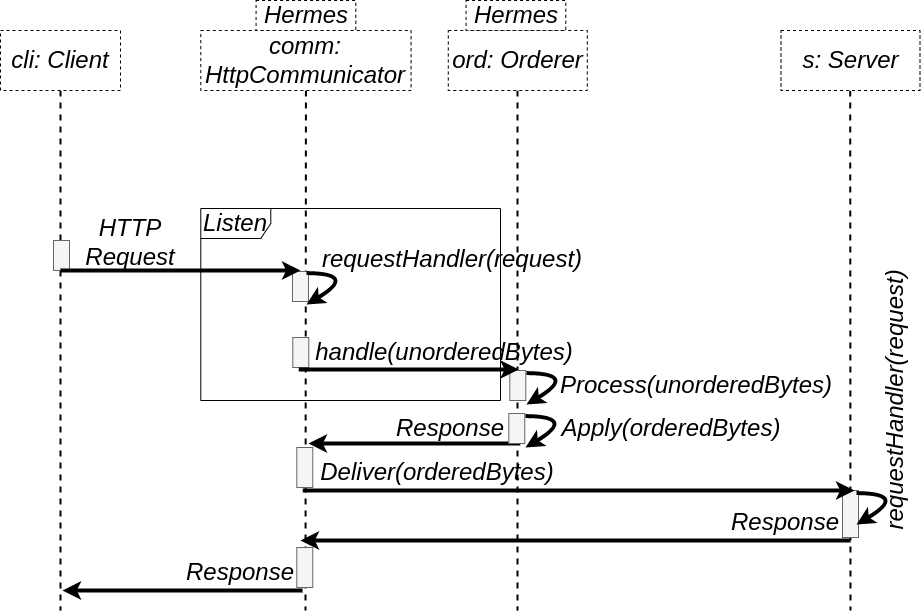
\includegraphics[width=\linewidth]{figures/deliver-listen-logic.drawio.png}
{\flushleft Fonte - Própria}
\label{fig:deliver-listen-logic}
\end{figure}

A Figura \ref{fig:deliver-listen-logic} mostra um diagrama do fluxo de informação passando pelos métodos \textit{Listen} e \textit{Deliver}. Uma vez que uma requisição HTTP qualquer é interceptada pelo Hermes, o evento Listen irá capturar essa requisição e transformar a requisição HTTP em \textit{bytes} e passar ao \textit{handler}. O \textit{handler} irá levar a informação em arranjo de bytes para ser ordenador pelo algoritmo de ordenação. Uma vez que o arranjo de \textit{bytes} está ordenado ele entra no método \textit{Deliver} e portanto eles já estão garantidamente ordenados.


\subsection{Experimentação}

Esta sessão trata como foram realizados as experimentações e, além disso, são mostrados as configurações para os experimentos.

\begin{figure}[htb!]
\centering
\caption{Representações das configurações sem replicação (A) e com ordenação respectivamente (B)}
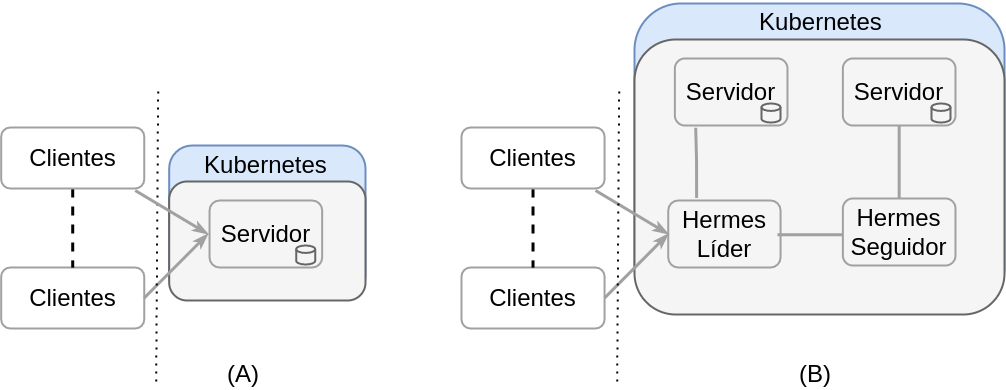
\includegraphics[width=\linewidth]{figures/confiuracoes-kubernetes.drawio.png}
{\flushleft Fonte - Adaptado de \textcite{renan2021hermes}}
\label{fig:arquitetura-cluster-ordenadores}
\end{figure}

\textit{Replicação com ordenação pelo interceptador:} A combinação para este cenário utiliza instâncias para gerador de carga, o servidor de armazenamento de \textit{logs}
sem consenso e o interceptador Hermes. Este cenário será utilizado para avaliar o custo médio de vazão de requisições HTTP.

\pagebreak

A Figura \ref{fig:arquitetura-cluster-ordenadores} (lado A) mostra a configuração do servidor sem replicação e a Figura \ref{fig:arquitetura-cluster-ordenadores} (lado B) mostra a configuração do servidor com replicação. Notar que o ordenador de mensagens fica à frente de cada réplica. Estas configurações foram usadas para os experimentos em ambiente real com implantação de orquestrador de contêineres. Este trabalho inclui duas aplicações que foram implementadas para os experimentos o \textit{HttpLogServer} e o \textit{HttpLogClient}, que serão explicadas a seguir. A aplicação \textit{HttpLogServer} tem basicamente 2 funções:

\begin{itemize}
\item Adicionar no fim de um arquivo (\textit{/tmp/logs/operations.txt}) as inserções via requisição POST.
\item Iterar sobre as linhas do arquivo \textit{/tmp/logs/operations.txt} e retornar a linha requerida via requisição GET.
\end{itemize}

Foi necessário implementar um servidor \gls{HTTP} customizado, usando as bibliotecas \textit{http.server} e \textit{sockethandler} para haver liberdade em registrar a contagem de requisições atendidas pelo servidor.

\subsection{Desenvolvimento}

O desenvolvimento do protocolo \gls{HTTP} foi feito em linguagem Go. O código atual do trabalho pode ser encontrado no Capítulo \ref{cap:conclusao}. Caso seja necessário alterar o código fonte, é recomendado alterar o nome do pacote Go, de `tonussi/hermes` para `xyz/hermes`. Também é recomendado criar um repositório no Github como `xyz/hermes`. Depois de alterar o nome do pacote Go, remova os arquivos \textit{go.mod} e \textit{go.sum} e execute as linhas a seguir:

\begin{verbatim}
go mod init github.com/xyz/hermes
go mod tidy
go get -u all
\end{verbatim}

\subsection{Detalhes de construção dos contêineres}

Para desenvolver no código se recomenda instalar o Docker Compose (define e executa contêineres Docker), o Docker (criador de imagens e contêineres de aplicação), Vscode (editor de código), \textit{make} (programa para executar comandos no Makefile), Makefile é um descritor de comandos úteis a serem executados pelo programa make. Uma vez instalados é possível apenas executar \textit{make build\_debug\_hermes}, para gerar imagem de contêiner para um Hermes com depurador Delve embutido. Fazendo isto deve ser possível acionar o modo Executar e Depurar selecionando a opção \textit{Debug Hermes (Attach)}, pois há um arquivo \textit{.vscode/launch.json} que integra o Delve com o Docker.

O Depurador indicará qual linha de código está sendo depurada. Como o Go é compilado, não é recomendado alterar o código e re-depurar imediatamente, então basta recompilar o código. O depurador Delve, ajuda a enxergar como o código está se comportando e, quais informações estão passado pelas funções.

Algumas notas importantes são, o arquivo Docker Compose irá gerar: um volume de dados para o BoltDB\footnote{BoltDB: \url{https://github.com/boltdb/bolt}} e um banco de dado usado internamente pelo Raft (interno ao Hermes). Por padrão o Hermes irá escutar o endereço \gls{IP}:8000 e enviar para o endereço \gls{IP}:8001.

O servidor da aplicação alvo poderá escutar no endereço \gls{IP}:8001. A menos que seja necessário alterar os endereços e portas, no caso se o servidor da aplicação precisar escutar outra porta, basta alterar o endereço de envio do Hermes via parâmetros.


% ---

\chapter{Avaliação Experimental}
\label{cap:experimentacao}

A avaliação foi sobre o Interceptador Hermes versão \gls{HTTP} e as aplicações: HttpLogClient e HttpLogServer. O HttpLogClient é um gerador de carga escrito em Python e tem a função de estressar o servidor da aplicação, enviando requisições HTTP. O HttpLogClient tem os seguintes parâmetros:

\begin{itemize}
\item \textit{address} do tipo \textit{TEXT}: define endereço do servidor;
\item \textit{port} do tipo \textit{INTEGER}: define porta do servidor;
\item \textit{bytes\_size} do tipo \textit{INTEGER}: define o tamanho da carga útil em número de bytes;
\item \textit{read\_rate} do tipo \textit{INTEGER}: define a taxa de leitura de 0 a 100 por cento;
\item \textit{n\_processes} do tipo \textit{INTEGER}: define número de processos do cliente;
\item \textit{thinking\_time} do tipo \textit{FLOAT}: define o tempo de reflexão entre as solicitações;
\item \textit{duration} do tipo \textit{FLOAT}: define a duração em segundos;
\end{itemize}

O HttpLogServer faz duas operações: \textit{get\_line(number)} (\textit{GET}) e \textit{append\_line(n-bytes-string)} (\textit{POST}). Estas funções são acionadas por requisições HTTP que podem ser realizadas pelos geradores de carga. Para acionar a função \textit{get\_line} basta enviar uma requisição \textit{GET} para \textit{/line/<number>}. Para acionar a função \textit{append\_line} basta enviar uma requisição \textit{POST} para \textit{/insert body: "128-byte-string"}. O \textit{HttpLogServer} tem os seguintes parâmetros:

\begin{itemize}
\item \textit{address} do tipo \textit{TEXT}: define endereço do servidor;
\item \textit{port} do tipo \textit{INTEGER}: define porta do servidor;
\end{itemize}

A função \textit{append\_line(n-byte-string)} é acionada por requisição \textit{POST} para \textit{/insert}, onde o corpo da mensagem é o conteúdo de uma \textit{string} de caracteres \gls{ASCII}, aleatória, e de tamanho parametrizável.
Em um primeiro momento foi necessário avaliar se os dados replicados corretamente, depois que foi visto que os \textit{logs} estavam sendo replicados, então começaram os experimentos de Latência (em nanosegundos) e, Vazão (número de requisições por segundo).

A avaliação se deu por examinar os dados brutos, para entender o comportamento do sistema perante algumas poucas cargas. A medida que se foi possível entender como aplicar cargas, foram feitos melhoramentos sobre os códigos do \textit{HttpLogServer} e \textit{HttpLogClient}.

Por exemplo o uso de \textit{Threads} em Python estava impedindo que os experimentos gerassem dados plausíveis, pois em Python não há concorrência real de \textit{Threads}. No entanto, o uso de Processos se apresentou como uma solução alternativa ao uso de \textit{Threads}.

\section{Medições}

\begin{figure}[htb!]
\centering
\caption{Esquematização de como e onde foram feitas as medições}
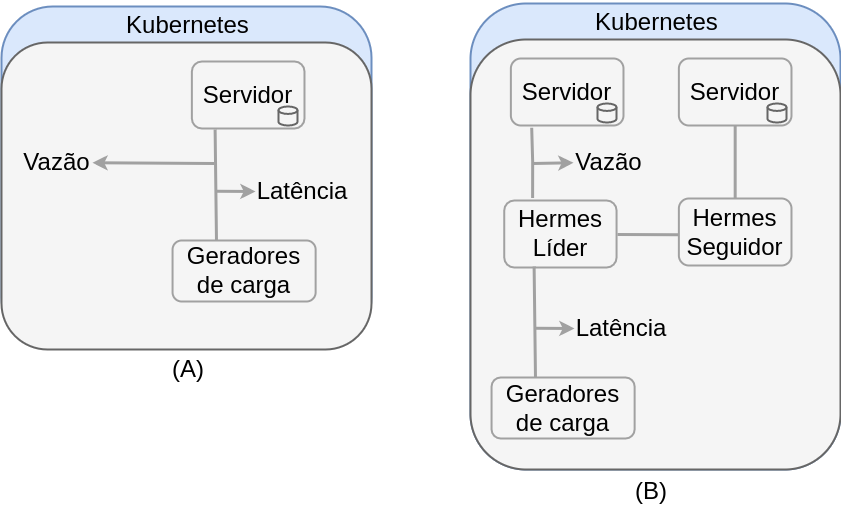
\includegraphics[width=0.8\linewidth]{figures/medicoes-configs.drawio.png}
{\flushleft Fonte - Própria.}
\label{fig:experimento-medicoes}
\end{figure}

A Figura \ref{fig:experimento-medicoes} ilustra em (A) que se trata de medições em um sistema sem replicação e em (B) que se trata de medições em um sistema replicado. Em (B), as entidades com nome \textit{Hermes Seguidor} representam 2 replicações, totalizando 3 réplicas juntamente com o Hermes Líder. A medição da vazão foi realizada como sendo a quantidade de requisições atendidas a cada segundo. A medição da latência foi feita como sendo o quanto tempo demora para executar uma requisição \gls{HTTP} e obter o retorno. As setas na figura (A) e (B) buscam mostrar onde o fluxo de informação foi capturado. Em (A) e (B) as latências são registradas no programa gerador de carga. Finalmente, em (A) e (B) as vazões são registradas no programa servidor sendo replicado.

\section{Ambiente de experimentação}

O ambiente de experimentação foi a plataforma Emulab\footnote{Emulab: \url{http://docs.emulab.net/}} \cite{emulab-10.1145/844128.844152}. Nesta plataforma foram alocadas 3 máquinas para os servidores de ordenação de mensagens e 2 máquinas para os geradores de carga. A máquina usada para os experimentos foi a d710. A especificações são as seguintes: marca Dell Poweredge R710, processador 2.4 GHz 64-bit Quad Core Xeon E5530 "Nehalem", cache de 8 MB L3, memória de 12 GB 1066 MHz DDR2 RAM (6 módulos de 2GB), discos rígidos de 500GB e 250GB 7200 rpm SATA.

% \begin{table}[htb!]
% \centering
% \caption{Máquinas usadas nos experimentos}
% \begin{tabular}{c|c|c|c|c}
% \textbf{Nome} & \textbf{Cores} & \textbf{Marca} & \textbf{Memória} & \textbf{Arquitetura} \\
% d430 & 8 & E5-2630v3 & 65536 & x86 64-bit \\
% d710 & 4 & Intel Quad Core Xeon E5530 & 12288 & x86 64-bit \\
% pc3000 & 1 & Xeon & 2048 & x86 64-bit \\
% \end{tabular}
% {\flushleft Fonte - Emulab}
% \label{tab:machines-emulab}
% \end{table}

\begin{figure}[htb!]
\centering
\caption{Esquematização dos nodos do Emulab}
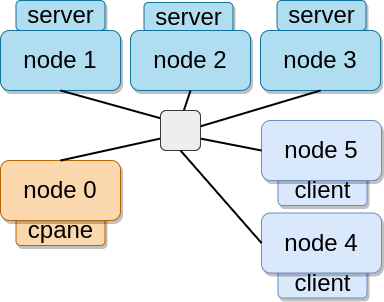
\includegraphics[width=0.45\linewidth]{figures/nodes.drawio.png}
{\flushleft Fonte - Própria.}
\label{fig:emulab-nodes}
\end{figure}

\pagebreak

A Figura \ref{fig:emulab-nodes} representa a configuração de nodos utilizada. A configuração apresentada mostra que foi pensado em deixar os servidores isolados, reduzindo ruídos. Alguns passos podem ser realizados para implantar um \textit{cluster} Kubernetes pronto para experimentação:

\begin{itemize}
\item É preciso instalar o Ansible\footnote{Ansible - \url{https://www.ansible.com/}} localmente.
\item Criar um experimento no Emulab e copiar os \textit{hosts}.
\item (Opcional) Listar os hosts no arquivo \textit{ansible/known\_hosts}.
\item (Opcional) Usar o \textit{script} \textit{scripts/ssh\_hosts.sh} para adicionar as chaves ssh. O script busca as interfaces de IP privada que serão usadas no passo do Kube Flannel. O script vai imprimir no terminal as interfaces e os IPs. Para configurar o Kube Flannel é necessário pegar apenas os IPs privados. IPs começando com \textsc{10.} são exemplos de IPs privados.
\item Configurar os \textit{hosts} do Emulab, em \textit{ansible/hosts}.
\item Configurar \textit{ansible\_user}, em \textit{ansible/hosts}.
\item Configurar o \textit{kubernetes/kube\_flannel.yaml} com os nomes das interfaces de rede privada que foram obtidas no passo anterior. Procurar por \textsc{--iface} no arquivo \textit{kubernetes/kube\_flannel.yaml}.
\item Executar o \textit{script} \textit{scripts/setup-emulab-cluster.sh}, para poder configurar o \textit{cluster} Kubernetes no Emulab. É preciso passar parâmetros para o script poder executar corretamente. Deve ser passado: caminho diretório Ansible; caminho diretório Kubernetes; nome do experimento no Emulab; nome do grupo no Emulab e a quantidade de servidores do tipo \textit{role=server}.
\item Instale o \textit{Kubectl} localmente, para poder executar os arquivos de descrição do Kubernetes.
\end{itemize}

\section{Caracterização da carga de trabalho utilizada}

O procedimento para capturar um conjunto de combinações de número de clientes e número de processos por cliente foi através de uma progressão sucessiva de carga, aumento do número de processos, variando o número de máquinas entre 1 e 2. Assim foi possível entender como a aplicação sem replicação estava se comportando com o aumento de carga. A mesma estratégia foi usada para a aplicação com interceptador Hermes à frente da aplicação.

% Os experimentos foram executados usando os parâmetros abaixo. Foi respeitado a ordem de execução dos experimentos. Para todos os casos abaixo foi mantido \textit{Thinking time} para os geradores de carga, após cada requisição, de 200ms, a duração total de cada experimento foi de 90s (gerando 90 segundos de medições de vazão no servidor). Como a troca de mensagens é via requisições HTTP o tamanho do corpo da mensagem foi definido como uma \textit{string} aleatória em ASCII de 128 bytes. Três casos principais foram analisados 100\% escrita (HTTP POST), 100\% leitura (HTTP GET) e, 50\% escrita com 50\% leitura.

% \begin{table}[!htb]
%     \caption{Combinações de cargas de trabalho}
%     \begin{center}
%     {
%         \begin{tabular}{
%             c|c|c
%         }
%         \cellcolor{gray!15} \textbf{Clientes} &
%         \cellcolor{gray!15} \textbf{Processos} &
%         \cellcolor{gray!15} \textbf{Total} \\
%         2 & 1 & 2 \\
%         1 & 4 & 4 \\
%         1 & 8 & 8 \\
%         2 & 4 & 8 \\
%         2 & 7 & 14 \\
%         2 & 8 & 16 \\
%         2 & 9 & 18 \\
%         2 & 10 & 20 \\
%         2 & 11 & 22 \\
%         2 & 12 & 24 \\
%         2 & 14 & 28 \\
%         1 & 30 & 30 \\
%         2 & 15 & 30 \\
%         1 & 32 & 32 \\
%         2 & 16 & 32 \\
%         2 & 32 & 64 \\
%         \end{tabular}
%     }
%     \end{center}
%     \label{tab:cargas}
%     % {\centering Fonte - Própria}
% \end{table}

O número total de processos simultâneos ao Hermes variou de 2 à 64. Cada rodada de experimento precisou de mais ou menos 45 segundos de pausa, para que não houvesse ruído em relação ao experimento anterior.

As marcas temporais, de cada medição foram registradas em nanosegundos para haver mais precisão. Gerar carga para apenas escrita via \gls{HTTP} POST se demonstrou mais consistente do que apenas leitura via \gls{HTTP} GET. O procedimento para extração dos pontos se dá por coletar durante 90 segundos a cada experimento.

\section{Avaliação de desempenho}

Esta sessão discute as configurações usadas em ambiente de testes e avalia o custo associado a utilização do interceptador Hermes.

Os experimentos forneceram dados, ponto a ponto. Os dados em determinado momento podem mostrar estagnação de vazão por unidade de tempo em relação à uma latência que só cresce porém com vazão estagnada. Isto pode sugerir a saturação do sistema. A avaliação final compara a saturação de dois cenários diferentes, com replicação e com ordenação via interceptador de mensagens.

Para determinar a saturação se observa a relação entre a latência dos geradores de carga enviando requisições ao Kubernetes. Um sistema saturado mantém conexões aguardando para serem atendidas demorando demais para entregar a resposta solicitada. Os componentes de software utilizados na execução dos experimentos foram:

\begin{itemize}
\item \textit{Servidor de armazenamento de log em disco:} Faz o papel de aplicação \textit{stateful} sendo replicada.
% , escrita em Python. Esta aplicação atende as funções: \textit{get\_line (line\_numer)} e \textit{append\_line (string)}. A função \textit{get\_line} itera sobre as linhas do arquivo e devolve ao cliente o conteúdo da linha requisitada. Já a função \textit{append\_line}, adiciona no fim do arquivo a nova \textit{string} no corpo da requisição POST.

\item \textit{Gerador de carga:} Faz o papel de cliente.
% , escrita em Python, que envia requisições HTTP, do tipo GET e POST, sendo que GET passa o número da linha desejada e, POST envia a \textit{string} a ser armazenada no arquivo em disco da aplicação servidora. A requisição GET irá invocar \textit{get\_line} no servidor, e as requisições POST irão invocar \textit{append\_line}. A \textit{string} enviada para \textit{append\_line} se trata de strings de quaisquer tamanho. Mas os geradores de carga, estão codificados para gerar strings de n-bytes de tamanho, sendo n um número inteiro parametrizável.

\item \textit{Hermes versão HTTP:} É o Interceptador e ordenador de mensagens HTTP.
\end{itemize}

\subsection{Resultados}

As comparações ocorreram entre um sistema sem replicação e um sistema replicado com ordenação de mensagens. As especificações das comparações estão listadas a seguir:

\begin{itemize}
\item Requisições GET (100\%), acionando \textit{get\_line} no servidor, 128 bytes strings, \textit{thinking time} de 200ms.
\item Requisições GET (50\%) e POST (50\%), acionando \textit{get\_line} e \textit{append\_line} no servidor, 128 bytes strings, \textit{thinking time} de 200ms.
\item Requisições POST (100\%), acionando \textit{append\_line} no servidor, 128 bytes strings, \textit{thinking time} de 200ms.
\end{itemize}

Os experimentos mostram as vazões médias em requisições por segundo no eixo $x$ e as latências dadas pelo nonagésimo percentil em milissegundos no eixo $y$. A seguir serão apresentados os gráficos comparativos dos experimentos.

\begin{figure}[htb!]
\centering
\caption{Requisição GET invocando a função \textit{get\_line} no servidor}
\includesvg[width=\linewidth]{figures/get-line.svg}
\label{fig:get-line}
\end{figure}

A Figura \ref{fig:get-line} mostra que nos pontos de 8-20 req/s o Hermes estava com aproximadamente 7 ms de latência, já no intervalo de 20 até 40 req/s o Hermes obteve latências próximos de 144 ms. O cenário sem replicação obteve latências em torno de 5 ms entre o período de 10 até aproximadamente 68 req/s. O Hermes apresentou consistência até 30 req/s, porém em aproximadamente 60 req/s ocorreu uma estagnação da vazão e crescimento da latência, o mesmo comportamento aconteceu para o sistema sem replicação, porém perto de 80 requisições por segundo. O cenário de 100\% requisições GET precisa que exista dados pre-populado com \textit{strings} de 128-bytes para que seja possível obter as linhas, 1000 linhas são pre-populadas e talvez isso faça que com o sistema Hermes obtenha vazão até 60 req/s e então estagne.

\begin{figure}[htb!]
\centering
\caption{Requisição GET/POST invocando as funções \textit{get\_line} e \textit{append\_line} no servidor}
\includesvg[width=\linewidth]{figures/get-append-line.svg}
\label{fig:get-append-line}
\end{figure}

A Figura \ref{fig:get-append-line} mostra que para o caso de 50\% GET e 50\% POST faz com que a vazão estagne antes de 60\%. Isto pode significar que no caso de 50\% GET 50\% POST é preciso preencher dados para haver vazão. Notar que em todos os cenários há pre-população de dados. O ponto de saturação do Hermes pode ser observado em aproximadamente 40 req/s, já o ponto de saturação no cenário sem replicação pode ser observado em aproximadamente 80 req/s.

As latências do Hermes se mantiveram aproximadamente 7 ms entre 8 até 20 req/s e a partir de 30 req/s a latência cresceu até aproximadamente 170 ms. Em 60 req/s a latência subiu e estagnou no ponto de 60 req/s. O cenário sem replicação obteve latências de aproximadamente 5 ms desde 10 req/s até aproximadamente 70 req/s e estagnou crescendo latência e obtendo vazões entre 70 e 80 req/s. O ponto de saturação do Hermes pode ser observado em aproximadamente 35 req/s, já o ponto de saturação no cenário sem replicação pode ser observado em aproximadamente 68 req/s.

\pagebreak

\begin{figure}[htb!]
\centering
\caption{Requisição POST invocando a função \textit{append\_line} no servidor}
\includesvg[width=\linewidth]{figures/append-line.svg}
\label{fig:append-line}
\end{figure}

A Figura \ref{fig:append-line} mostra que o Hermes obteve latências de aproximadamente 7 ms entre o período de 10 até aproximadamente 70 req/s. Entre 70 e 80 req/s o Hermes apresentou estagnação da vazão enquanto a latência aumentou para 225 ms. O cenário sem replicação obteve latências de aproximadamente 5 ms entre 10 até aproximadamente 80 req/s. Em 80 req/s começou a estagnar a vazão de requisições, subindo a latência até aproximadamente 200 ms. O ponto de saturação do Hermes pode ser observado em aproximadamente 68 req/s, já o ponto de saturação no cenário sem replicação pode ser observado em aproximadamente 78 req/s.

Em geral, há sobrecarga ao usar o Hermes. A sobrecarga foi baixa no cenário 100\% \textit{POST}, que é um comportamento \textit{append-only}, onde apenas se adiciona uma linha no fim do arquivo de (\textit{log}). O custo da latência em ms fica bastante elevado com a presença de comandos \textit{GET}.

% Usei com percentil 90

% Fonte: https://docs.google.com/spreadsheets/d/1zIB5y5vrI235vU2fl7WXTsgDcKqYfjnukTRzEOGMWEg/edit#gid=751333503 (latência percentil 90)

% Usei com percentil 90

% ---
% 4 - Conclusão
% ---
\phantompart
\chapter{Conclusão}
\label{cap:conclusao}

A presente monografia apresentou uma forma de comunicação via HTTP para o interceptador e ordenador de mensagens, Hermes. Esta forma de comunicação permite que aplicações que trabalham com HTTP, possam ser replicadas. Os desenvolvedores podem focar na lógica de negócio da sua aplicação ou \gls{API}, sem se preocuparem com detalhes de ordenação. Este trabalho é também, um estudo sobre: a arquitetura geral do interceptador Hermes; técnicas de ordenação, orquestradores de contêineres, algoritmos de consenso e tópicos relacionados.

O experimentos no Emulab mostraram detalhes sobre a implantação do Hermes, e como operar com ele à frente de uma aplicação feita em Python. Vale lembrar que o uso de orquestrador de contêineres é necessário para tornar operacional o Hermes. A aplicação Python salva as operações dos usuários em \textit{log} no disco. A partir das análises dos experimentos foi possível concluir que o Hermes obteve sobrecarga em relação ao sistema sem replicação.

O uso de técnicas de ordenação de mensagens mostrou que um sistema se mantêm operacional a despeito de uma certa quantidade de falhas das réplicas do serviço, além de oferecer melhor escalabilidade ao serviço replicado. A implementação da interface \textit{communicator} em Go mostrou que protocolos de aplicação (\gls{HTTP}) podem ser integrados ao sistema de ordenação de mensagens. Os experimentos sem replicação mostram latências menores e mantêm vazões altas por mais pontos de experimentos.

Os experimentos com o ordenador Hermes mostraram latências mais altas em relação ao sistema sem replicação. As leituras em arquivo de uma linha aleatória a cada requisição \textit{GET} fazem com que os gráficos mostrem que o servidor consegue responder em baixas latências até determinada implicação de carga, mas sobe abruptamente em certo ponto. Durante os experimentos, foram feitas diversas tentativas de coleta de pontos e foram criados várias configurações de experimentação, porém os resultados sempre estavam culminando para algo parecido. Contudo, a escrita em arquivo pela requisição POST se demostrou mais previsível nos gráficos, aparentando uma subido gradual da latência enquanto a vazão estagnava. O código usado para este trabalho pode ser encontrado em \url{https://github.com/tonussi/tcc.git}.

\section{Trabalhos Futuros}

Existe espaço para explorar novas funcionalidades e adicionar integração com novos algoritmos de ordenação de mensagens.

% Uma possibilidade de melhoria é na parte de garantia de que os dados escritos em disco estejam sincronizados em caso de replicas falharem e se recuperarem. Pois nos experimentos, notou-se que devido a sobrecarga dos \textit{Nodes} ocorria a falta de um ou outro \textit{Pod} e precisava ser reiniciado. Uma vez que o \textit{Pod} era reiniciado os \textit{logs} das operações não se encontravam iguais. No entando, o foco deste trabalho não era recuperação em caso de falha.

\textit{Adição de novos protocolos de comunicação:} Por exemplo a implementação do \textit{protocolo \gls{UDP}} está em aberto para permitir entregas não baseadas em conexão. 
% Existe um código iniciado por \textcite{renan2021hermes}, porém ainda não foi finalizado e experimentado. Até o presente trabalho os protocolos TCP e HTTP foram implementados.

\textit{Aprimorar o serviço de ordenação proposto em \textcite{renan2021hermes}:} De maneira geral, pode-se mencionar a implementação de diferentes protocolos de comunicação de ordenação de mensagens, assim como no desenvolvimento de estratégias para aumento da vazão na entrega de requisições às réplicas.

% \textit{Implementar \gls{RME} como um microsserviço:} Este objetivo visa utilizar o serviço de ordenação de mensagens proposto por \textcite{renan2021hermes} para implementar um serviço completo de \gls{RME}. Com esse serviço, espera-se que desenvolvedores de aplicações possam se beneficiar de redundância e maior disponibilidade dos seus serviços sem ter que implementar aspectos específicos de tolerância a falhas.

% \textit{Desenvolver um protótipo do serviço \gls{RME} no topo do orquestrador de contêineres Kubernetes:} Este protótipo permitirá observar a aplicabilidade e transparência do serviço na prática e observar os desafios e limitações da configuração da infraestrutura e do serviço.

\textit{Novos protocolos de consenso no Hermes:} Há a possibilidade de inclusão de outros protocolos de consenso, como: Paxos \cite{lamport1998part}, Calvin \cite{calvin-10.1145/2213836.2213838}, CRDT \cite{demers1987epidemic}, dentre outros que podem ser encontrados em \url{https://github.com/heidihoward/distributed-consensus-reading-list}.

\textit{Ordenação em lotes:} Esta estratégia de ordenação em lotes pode requerer uma terceira fonte de informação, também replicada. Esta fonte guardaria o conteúdo das requisições em bytes com uma chave associada ao lote e uma vez que o ordenador Hermes agrupasse um lote de um tamanho determinado, faria-se então a ordenação de um lote pela chave. Depois de ordenar a chave, recupera-se o lote da fonte de informação e se aplica o lote nas réplicas.

\textit{Mudança de líder no sistema Raft do Hermes}: Possibilitar que o líder mude, caso ocorra falha do \textit{Pod} que segura o Hermes Líder (nó do Raft atuando como líder). É possível, e aparentemente viável, que essa mudança permita que o sistema de \textit{Load Balancer} do Kubernetes seja integrado ao sistema Hermes. Por enquanto o Hermes líder é fixo, e atua como \textit{Node Port}.

\textit{Otimização do atendimento de requisições HTTP:} As requisições HTTP do tipo GET, POST, \textit{etc.} podem ter uma resposta do servidor de aplicação. Porém encarregar o Hermes de responder ao cliente pode causar um atraso no processamento de ordenação de mensagens. Sabendo disto, existe espaço para repensar no mecanismo de resposta após aplicar uma mensagem no servidor replicado. Poderia haver um outro serviço que disponibiliza a resposta do servidor em um outro canal de comunicação.


% ----------------------------------------------------------
% ELEMENTOS PÓS-TEXTUAIS
% ----------------------------------------------------------
\postextual
% ----------------------------------------------------------

% ----------------------------------------------------------
% Referências bibliográficas
% ----------------------------------------------------------
\begingroup
\printbibliography[title=REFERÊNCIAS]
\endgroup

% ----------------------------------------------------------
% Glossário
% ----------------------------------------------------------
% \imprimirglossario

% ----------------------------------------------------------
% Apêndices
% ----------------------------------------------------------

% ---
% Inicia os apêndices
% ---
\begin{apendicesenv}
% \partapendices* 
% ----------------------------------------------------------
\chapter{Descrição 1}
% ----------------------------------------------------------

Textos elaborados pelo autor, a fim de completar a sua argumentação. Deve ser precedido da palavra APÊNDICE, identificada por letras maiúsculas consecutivas, travessão e pelo respectivo título. Utilizam-se letras maiúsculas dobradas quando esgotadas as letras do alfabeto. 

\end{apendicesenv}
% ---


% ----------------------------------------------------------
% Anexos
% ----------------------------------------------------------

% ---
% Inicia os anexos
% ---
\begin{anexosenv}
%	\partanexos*
\chapter{Anexo - Artigo do Projeto}

\pagebreak

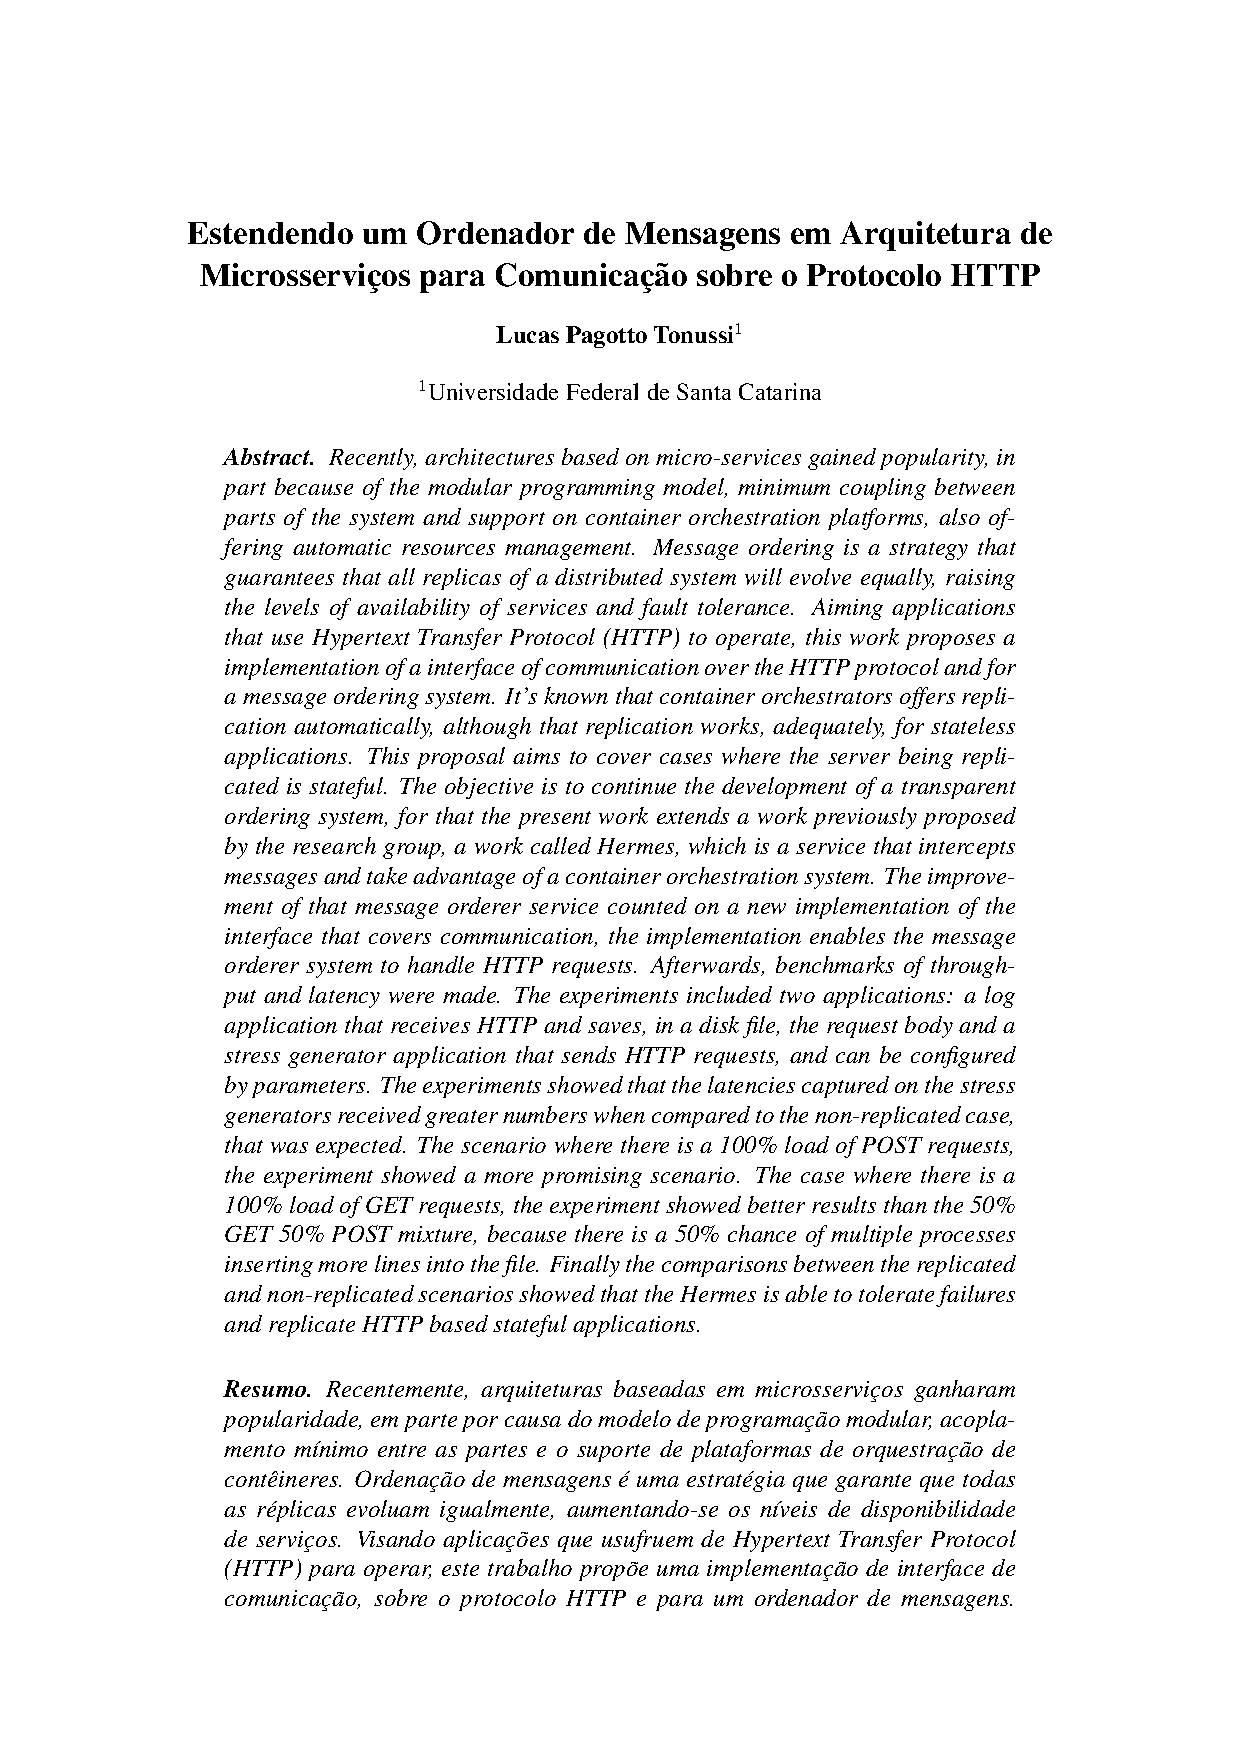
\includepdf[pages={1-},scale=1]{aftertext/sbc_odorico_github.pdf}

\end{anexosenv}

%---------------------------------------------------------------------
% INDICE REMISSIVO
%---------------------------------------------------------------------
% \phantompart
% \printindex
%---------------------------------------------------------------------

\end{document}
